\documentclass[a4paper,oneside,12pt]{book}
%% === nezbytné balíčky:
\usepackage[IL2]{fontenc} 
\usepackage[utf8]{inputenc} % vstupní znaková sada UTF-8 

\usepackage[backend=biber,
			sorting=nty,
			style=ieee]{biblatex}
\addbibresource{bibliographyExport.bib}

\usepackage[english]{babel}

\usepackage{pdfpages} % pokud nemáte formulář "Zadání bak./dipl. práce" naskenovaný jako PDF, tak ZAKOMENTUJTE

%\usepackage{encxvlna} % postará se o spojky a předložky, které dle českých pravidel nesmí být na konci řádku. Dokumentace: http://texdoc.net/texmf-dist/doc/generic/encxvlna/encxvlna.pdf

\usepackage[a4paper, hmarginratio=1:1]{geometry} % využití celé A4 stránky a nastavení okrajů, pro OBOUSTRANNÝ TISK

%% === balíčky, které se mohou hodit:
\usepackage[hidelinks,breaklinks]{hyperref} % v PDF budou klikací odkazy ("hidelinks" je nebude rámovat)
\usepackage{graphicx} % balíček pro vkládání RASTROVÝCH grafických souborů (PNG apod.)
%\usepackage{epsfig} % balíčky pro vkládání VEKTOROVÝCH grafických souborů typu EPS

%\usepackage{float} % rozšířené možnosti umístění obrázků
%\usepackage{caption} % pro popisky obrázků, tabulek atd.

\usepackage{tabularx} % rozšířené možnosti tabulek
%\usepackage{tabu} % jiný balík pro rozšířené možnosti tabulek

\usepackage{listings}  % balíček vhodný pro ukázky kódu 
\usepackage{amsmath} % balíček pro pokročilou matematickou sazbu
%\usepackage{color} % pro možnost barevného textu
%\usepackage{fancybox} % umožňuje pokročilé rámečkování
%\usepackage{index} % nutno použít v případě tvorby rejstříku balíčkem makeindex
%\newindex{default}{idx}{ind}{Rejstřík} % zavádí rejstřík v případě použití balíku index


\topmargin=-15mm      % horní okraj trochu menší
\textwidth=150mm      % šířka textu na stránce
\textheight=240mm     % "výška" textu na stránce

%\frenchspacing % za větou bude mezislovní mezera (v anglických textech je mezera za větou delší)
\widowpenalty=1000 % "síla" zákazu vdov (= jeden řádek odstavce na konci stránky)
\clubpenalty=1000 % "síla" zákazu sirotků (= jeden řádek slovo odstavce samostatně na začátku stránky)
\brokenpenalty=1000 % "síla" zákazu zlomu stránky za řádkem, který má na konci rozdělené slovo

\pagenumbering{arabic} % číslování stránek arabskými číslicemi
\pagestyle{plain}      % stránky číslované dole uprostřed

\parindent=0pt % odsazení 1. řádku odstavce
\parskip=7pt   % mezera mezi odstavci

\newcommand{\ti}{\textit} % zkrácený příkaz pro kurzívu
\newcommand{\tb}{\textbf} % zkrácený příkaz pro tučné písmo


%% --- zde jsou makra, tj. "konstanty" - některé musíte změnit! --- %%
\newcommand{\cvut}{Czech Technical University in~Prague}
\newcommand{\fjfi}{Faculty of Nuclear Sciences and Physical Engineering}
\newcommand{\katedra}{Department of Software Engineering}
\newcommand{\katedraKLFF}{Department of plasma physics and fotonics}
\newcommand{\program}{Applications of Informatics in Natural science} % změňte, pokud máte jiný stud. program
\newcommand{\spec}{--} % změňte, pokud studijní program má specializaci

\newcommand{\druh}{Master thesis} % nebo "Diplomová práce"
\newcommand{\woman}{} % pokud jste ŽENA, ZMĚŇTE na: ...{\woman}{a} (je to do Prohlášení)

\newcommand{\logoCVUT}{
\includegraphics{symbol_cvut_konturova_verze_cb.pdf}} % logo ČVUT -- podle grafického manuálu ČVUT platného od prosince 2016. Pokud nevyhovuje PDF-verze, tak použijte jinou variantu loga: https://www.cvut.cz/logo-a-graficky-manual -> "Symbol a logo ČVUT v Praze"). Pokud chcete logo úplně vynechat, zadejte místo "\includegraphics{...}" text "\vspace{35mm}"

% přesně podle formuláře "Zadání bak./dipl. práce" VYPLŇTE:
\newcommand{\nazevcz}{Modelování laserovej absorpce pomocí metod strojového učení}    % český název práce (přesně podle zadání!)
\newcommand{\nazeven}{Modelling laser absorption using machine learning methods}          % anglický název práce (přesně podle zadání!)
\newcommand{\autor}{Bc. Samuel Šitina}   % vyplňte své jméno a příjmení (s akademickým titulem, máte-li jej)
\newcommand{\vedouci}{doc. Ing. Ondřej Klimo, Ph.D.} % vyplňte jméno a příjmení vedoucího práce, včetně titulů, např.: Doc. Ing. Ivo Malý, Ph.D.
\newcommand{\pracovisteVed}{\katedraKLFF, \fjfi, \cvut} % ZMĚŇTE, pokud vedoucí Vaší práce není z KSI
\newcommand{\konzultant}{--} % POKUD MÁTE určeného konzultanta, NAPIŠTE jeho jméno a příjmení + tituly
\newcommand{\pracovisteKonz}{--} % POKUD MÁTE konzultanta, NAPIŠTE jeho pracoviště

% podle skutečnosti VYPLŇTE:
\newcommand{\rok}{2024}  % rok odevzdání práce (jen rok odevzdání, nikoli celý akademický rok!)
\newcommand{\kde}{Praze} % studenti z Děčína ZMĚNÍ na: "Děčíně" (doplní se k "prohlášení")

\newcommand{\klicova}{Klíčová slova}   % zde NAPIŠTE česky cca 3-5 klíčových slov
\newcommand{\keyword}{Key words}       % zde NAPIŠTE anglicky cca 3-5 klíčových slov (přeložte z češtiny, ale odborně)
\newcommand{\abstrCZ}{Popis práce česky}    % zde NAPIŠTE abstrakt v češtině (alespoň 7 vět, min. 80 slov. Pokuste se, aby CZ i EN abstrakt nezpůsobily přetečení strany 6 na stranu 7, tj. aby se obojí i s klíčovými slovy vešlo na JEDNU stránku)
\newcommand{\abstrEN}{Popis práce anglicky} % zde NAPIŠTE abstrakt v angličtině

\newcommand{\prohlaseni}{Hereby I declare that this thesis is my original authorial work, which I have worked out on my own with the guidance of my supervisor. All sources, references, and literature used or excerpted during the elaboration of this work are properly cited and listed in complete reference to the due soruce.}

\newcommand{\podekovani}{I would like to thank my supervisor Doc. Ing. Ondřej Klimo, Ph.D. for valuable guidance throughout the entire process. I would like to thank my parents who have supported unconditionally me in unimaginable ways. I would also like to thank my sister and my brother, whose advice helped me find motivation in the times of struggle.}


\begin{document}
%%%%%%%%%%%% TITULNÍ STRANA -- následujících cca 30 řádků se generuje AUTOMATICKY. Neměňte!!! Výjimka: práce psané v angličtině! %%%%%%%%%%%%
\thispagestyle{empty}

\begin{center}
    {\Large \textsc{\cvut}\\[4mm] \textsc{\fjfi}}\par
    \vspace{4mm}

    \begin{tabular}{rl}
		\tb{Department:} & \tb{\katedra}\\
		\tb{Study programme:} & \tb{\program}\\
    \end{tabular}

   \vspace{10mm} \logoCVUT \vspace{15mm} 

   {\huge \tb{\nazeven}\par}
   \vspace{5mm}
   
   \vspace{15mm}
   {\Large \MakeUppercase{\druh}}

   \vfill
   {\large
    \begin{tabular}{ll}
  	Author: & \autor\\
   	Supervisor: & \vedouci\\
   	Year: & \rok
    \end{tabular}
   }
\end{center}

%%%%%%%%%%%% ZADÁNÍ PRÁCE %%%%%%%%%%%%
% Zadání (podepsané děkanem atd.) dostanou studenti KSI od sekretářky (nebo ji požádají, např. e-mailem).
\newpage  % SEM NESAHEJTE!
\thispagestyle{empty} % SEM NESAHEJTE!

%% naskenované ZADÁNÍ PRÁCE (nechte odkomentovanou jednu možnost!):
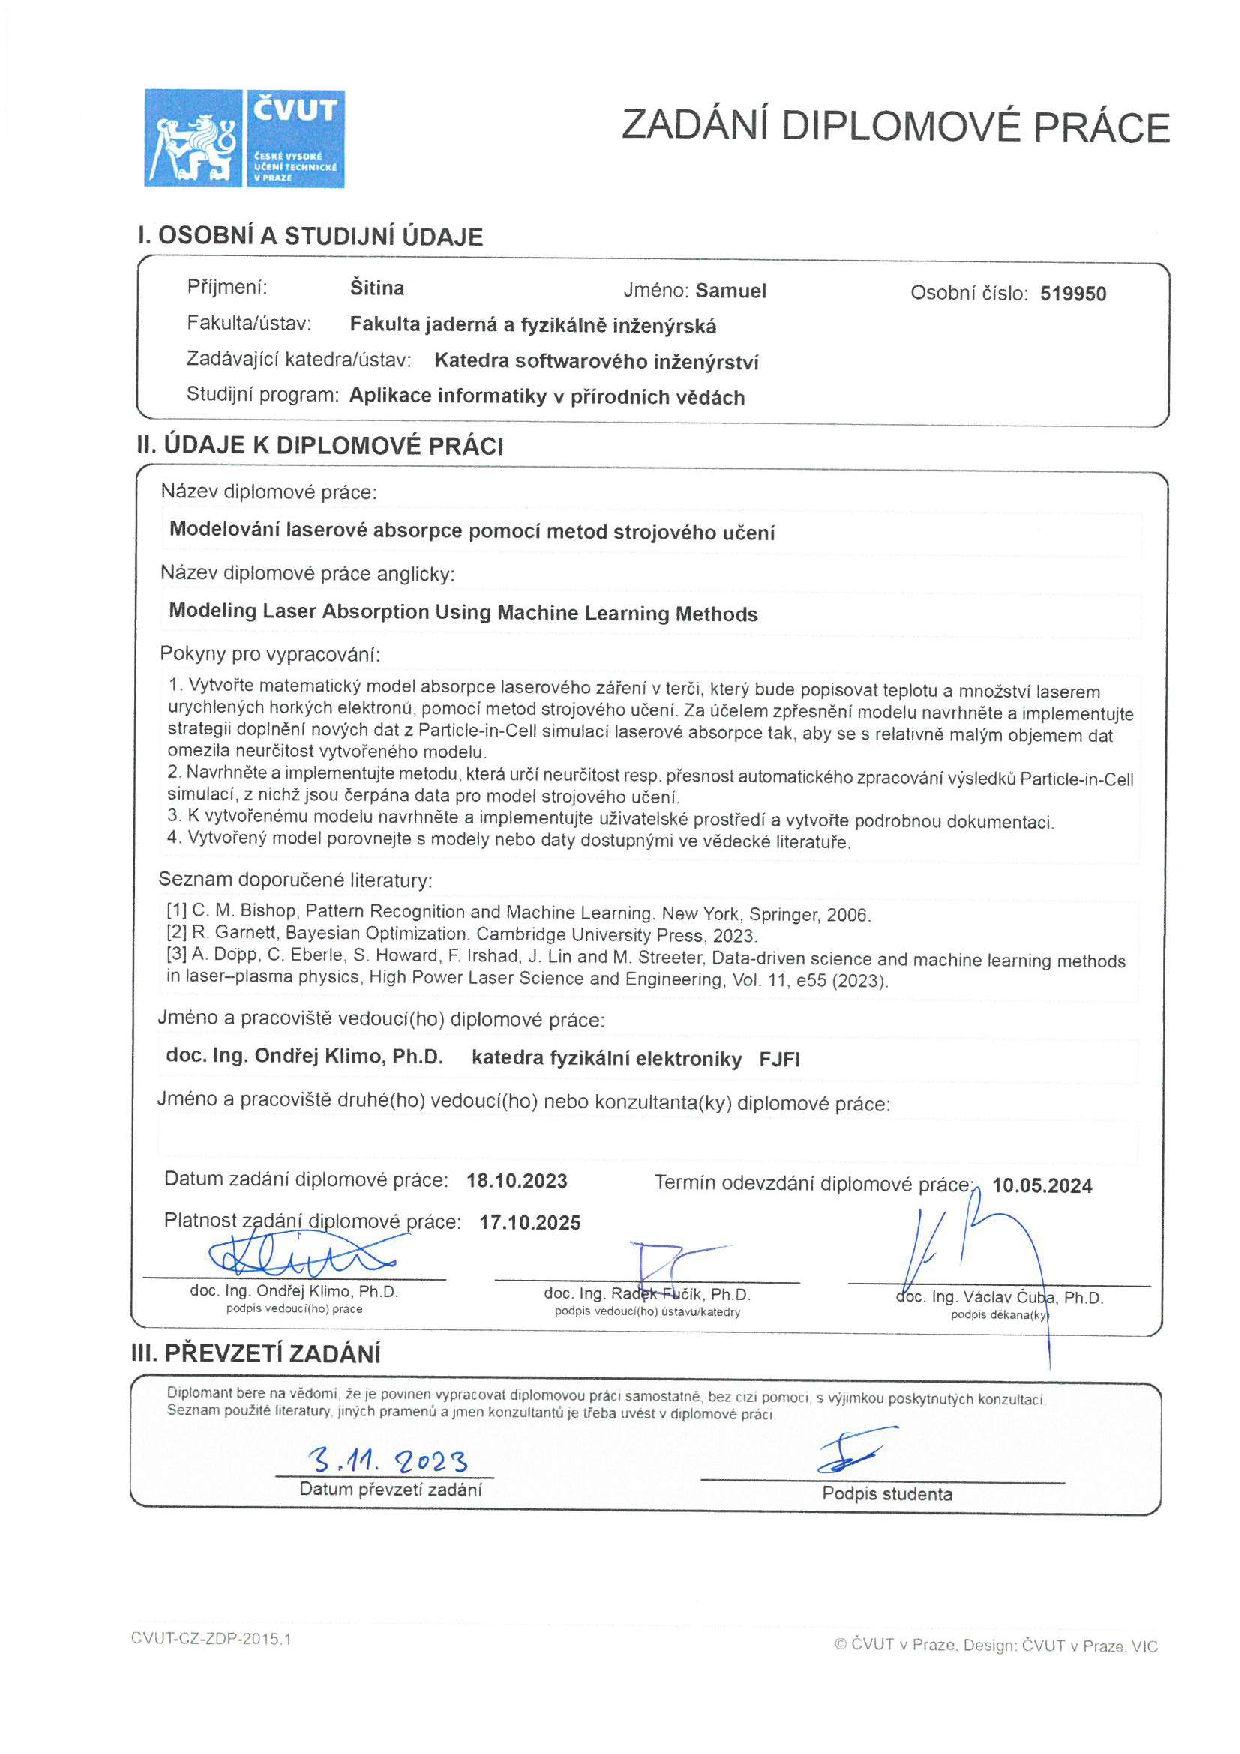
\includepdf[pages={1,2}]{zadani_cele.pdf} % PDF má 2 stránky


%%%%%%%%%%%% Prohlášení -- SEM NESAHEJTE! Generuje se automaticky z výše nastavených maker \kde{} a \prohlaseni{}. %%%%%%%%%%%%
\newpage % SEM NESAHEJTE!
\thispagestyle{empty}  % SEM NESAHEJTE!

~ % SEM NESAHEJTE!
\vfill % prázdné místo. SEM NESAHEJTE!

\tb{Statement of originality}

\vspace{1em} % vertikální mezera. SEM NESAHEJTE!
\prohlaseni

\vspace{2em}  % SEM NESAHEJTE!
\hspace{-0.5em}\begin{tabularx}{\textwidth}{X c}  % SEM NESAHEJTE!
In Prague on .................... &........................................ \\	% SEM NESAHEJTE!
	& \autor
\end{tabularx}	% SEM NESAHEJTE!


%%%%%%%%%%%% Poděkování -- tuto stránku můžete celou odstranit %%%%%%%%%%%%
\newpage
\thispagestyle{empty}

~
\vfill % prázdné místo

\tb{Acknowledgment}

\vspace{1em} % vertikální mezera
\podekovani
\begin{flushright}
\autor
\end{flushright}  % <------- tady končí stránka s poděkováním


%%%%%%%%%%%% ABSTRAKT atp. Je generován AUTOMATICKY podle maker nastavených na začátku souboru) %%%%%%%%%%%% 
\newpage   % SEM NESAHEJTE!
\thispagestyle{empty}   % SEM NESAHEJTE!

% příprava:    (na následujících 8 řádků NESAHEJTE!)
\newbox\odstavecbox
\newlength\vyskaodstavce
\newcommand\odstavec[2]{%
    \setbox\odstavecbox=\hbox{%
         \parbox[t]{#1}{#2\vrule width 0pt depth 4pt}}%
    \global\vyskaodstavce=\dp\odstavecbox
    \box\odstavecbox}
\newcommand{\delka}{120mm} % šířka textů ve 2. sloupci tabulky

% použití přípravy:    % dovnitř "tabular" vůbec NESAHEJTE!
\begin{tabular}{ll}
  {\em Title:} & \odstavec{\delka}{\nazeven} \\[2em]
  {\em Author:} & \autor \\[1em]
  {\em Study programme:} & \program \\[1em]
  {\em Type of thesis:} & \druh \\[1em]
  {\em Supervisor:} & \odstavec{\delka}{\vedouci\ \pracovisteVed} \\
    
  \multicolumn{2}{l}{\odstavec{\textwidth}{{\em Abstract:} ~ \abstrEN  }} \\[1em]
  {\em Key words:} & \odstavec{\delka}{\klicova} \\[2em]

  {\em Title:} & ~\\
  \multicolumn{2}{l}{\odstavec{\textwidth}{\bf \nazeven}}\\[1em]
  {\em Author:} & \autor \\[1em]
  \multicolumn{2}{l}{\odstavec{\textwidth}{{\em Abstract:} ~ \abstrCZ  }} \\[1em]
  {\em Key words:} & \odstavec{\delka}{\keyword}
\end{tabular}



%%%%%%%%%%%% Obsah práce ... je generován AUTOMATICKY %%%%%%%%%%%%
\newpage  % SEM NESAHEJTE!
\parskip=0pt
\tableofcontents % SEM NESAHEJTE!
\parskip=7pt
\newpage % SEM NESAHEJTE!


%--------------------------------------------------------
%|         Zde začíná SAMOTNÁ PRÁCE (text)              |
%--------------------------------------------------------


\chapter*{Introduction}
\addcontentsline{toc}{chapter}{Introduction}


Plasma, the fourth state of matter, makes up more than 99\% of the visible universe~\cite{plasma-intro}. It has been observed in technology since 1810 in various cases of electrical discharge, but a deeper study of plasma has begun in the 1950s in the context of a controlled nuclear fusion. Later, with the development of high-powered lasers, it became possible to create a plasma with densities similar to those of solids.

Advancements in laser technology have enabled us to study plasma under increasingly extreme conditions. In parallel, computer simulations offer a complementary method, allowing us to explore specific effects from the first principles. However, for some applications, surrogate models may be more appropriate. These models focus solely on describing the relationship between inputs and outputs, without incorporating the underlying physical principles.

In this thesis, we create a surrogate model for laser absorption in high-intensity short-pulse laser-plasma interactions. We explore a segment of the parameter space using several hundred particle-in-cell simulations and model the hot electron temperature based on these parameters. This multi-step process is presented in detail throughout the thesis.

In the first chapter, we introduce the fundamental physical effects relevant to the studied problem, providing the necessary background to understand the data obtained from simulations. This chapter also covers the motivation behind this work and discusses key aspects of particle-in-cell simulations.

Chapter 2 focuses on retrieving the hot electron temperature from the simulation results. We aim for an unsupervised process, which facilitates the addition of more simulations in the future by automating the procedure. Various fitting methods are reviewed for estimating the parameters without supervision and one explicit method is explained.

In Chapter 3, we discuss three potential surrogate models suitable for this thesis. Although we do not implement these models ourselves, we explain the underlying principles on which they are based.

The fourth chapter is dedicated to implementing the fitting method introduced in Chapter 2. We address the challenges encountered when processing large amounts of simulation data, examine the strengths and weaknesses of the proposed fitting method, and compare the results to what we consider reliable estimates of fit parameters.

Chapter 5, the final chapter, centers on applying the models discussed in Chapter 3. We compare the performance of these models on the dataset analyzed in Chapter 4, present a tool for visually inspecting the models, and propose a strategy for expanding the dataset by running additional simulations.

This comprehensive approach aims to create a robust surrogate model for better understanding laser-plasma interactions in certain part of the parameter space with possible application in optimizing the X-ray photon yields.  We try to maximize the use of both simulation data and advanced modelling techniques.


\chapter{Plasma}
A plasma is a quasi-neutral gas of charged and neutral particles which exhibits collective behaviour \cite{plasma-intro3}. In simple terms, quasi-neutrality means that the density of electrons $n_e$ and density of positively charged ions $n_i$ locally satisfy:
\begin{equation}
	n_e \simeq Zn_i
\end{equation}
\noindent where $Ze$ is the charge of one positively charged ion and $e$ is elementary charge \cite{plasma-intro}. 

The non-neutral particles in plasma are subject to electric and magnetic fields generated either by external sources or by neighbouring particles. The long-range nature of Coulomb potential ensures that macroscopic fields dominate over forces created by microscopic fluctuations \cite{plasma-intro}. To explain the collective behaviour properly, one can start by writing \textit{Vlasov equation} \cite{laser-plasma4}:
\begin{equation}
	\frac{\partial f_j}{\partial t} + \bm{v} \cdot \frac{\partial f_j}{\partial \bm{x}} + \frac{q_j}{m_j}\left(\bm{E} + \frac{\bm{v}\times\bm{B}}{c}\right)\cdot \frac{\partial f_j}{\partial \bm{v}} = 0
\end{equation}
\noindent where $f_j = f_j\left(\bm{x},\bm{v},t\right)$ is the phase space distribution function, which characterizes the location of the particles of species $j$ (electrons or ions) in phase space $\left(\bm{x},\bm{v}\right)$ (position, velocity) as a function of time. $q_j$ and $m_j$ are charge and mass of the species $j$ and $c$ is the speed of light \cite{laser-plasma4}.

After calculating the 0th and 1st moment of Vlasov equation (averaging through $\bm{v}$), we obtain the equation of continuity and force equations for the density $n_j = \int f_j\left(\bm{x},\bm{v},t\right)\mathrm{d}\bm{v}$ and mean velocity $\bm{u}_j$ defined by $n_j\bm{u}_j = \int \bm{v} f_j\left(\bm{x},\bm{v},t\right)\mathrm{d}\bm{v}$:
\begin{equation}
	\label{eq:continuity}
	\frac{\partial n_j}{\partial t} + \nabla\cdot\left(n_j \bm{u}_j\right) = 0
\end{equation}
\begin{equation}
	\label{eq:momentum}
	n_j \left(\frac{\partial \bm{u}_j}{\partial t} + \left(\bm{u}_j\cdot\nabla\right)\bm{u}_j\right) = \frac{n_j q_j}{m_j}\left(\bm{E} + \frac{\bm{u}_j\times\bm{B}}{\mathrm{c}}\right) - \frac{1}{m_j}\nabla p_j
\end{equation}
\noindent where $p_j$ is isotropic pressure and in case of negligible heat flow also the adiabatic state equation:
\begin{equation}
	\label{eq:energy}
	p_jn_j^{-\gamma} = \mathrm{const.}.
\end{equation}
\noindent where $\gamma = \left(2+N\right)/N$ and $N$ is the number of degrees of freedom. Equations \ref{eq:continuity}, \ref{eq:momentum} and \ref{eq:energy} together with the Maxwell equations are often referred to as \textit{two-fluid model of plasma} and describe wide range of plasma (collective) behaviour such as plasma waves or Debye shielding \cite{laser-plasma4}.

\section{Temperature of plasma}
\label{sec:temperature-intro}
In this thesis, we are studying so called \textit{hot electrons} produced by the interaction of short laser pulse of high intensity with plasma. All important details of the physical phenomena will be covered in later sections, but let us now look at what is meant by $hot$ and how the temperature of plasma is usually understood.

In a gas in the thermal equilibrium, particles velocities are given by Maxwellian distribution (in three dimensions) \cite{plasma-intro3}:
\begin{equation}
	f(\bm{v}) = n\left(\frac{m}{2\pi \boltz}\right)^{3/2}\exp\left(-\frac{\frac{1}{2}m v^2}{\boltz T}\right)
\end{equation} 
\noindent where $v = \norm{\bm{v}}$ is magnitude of velocity, $m$ is mass. $\boltz$ is the Boltzmann constant and $T$ is temperature. The average kinetic energy $E_{av}$ is then \cite{plasma-intro3}:
\begin{equation}
	E_{av}=\frac{3}{2}\boltz T
\end{equation}
Because of this relation between $E_{av}$ and $T$, it is customary in plasma physics to express the temperature in the same units as energy. If $\boltz T = 1 \, \mathrm{eV} = 1.6 \times 10^{-19}\, \mathrm{J}$, then \cite{plasma-intro3}:
\begin{equation}
	T = \frac{1.6 \times 10^{-19}}{1.38\times 10^{-23}}=11600
\end{equation}
\noindent From this it follows that the factor of the conversion is:
\begin{equation}
	1 \mathrm{eV} = 11600\,\mathrm{K}
\end{equation} 
The electrons and the ions can have different temperature \cite{plasma-intro3}. Moreover, there can be multiple groups of electrons with different distributions, but we will describe this more deeply in one of the later sections.

\subsection*{Critical density}
Now consider a high frequency electric field $\bm{E} = \bm{E(x)}\exp\left(-i\omega t\right)$. The frequency $\omega$ is assumed to be greater than electron plasma frequency $\omega_{\mathrm{pe}}$ defined as $\omega_{\mathrm{pe}}^2=4\pi e^2 n_\mathrm{e}/m_\mathrm{e}$ with $n_\mathrm{e}=Zn_{i}$ being electron density and $m_\mathrm{e}$ electron mass. Maxwell equations plus equation of motion of electron fluid give us:
\begin{equation}
	\nabla \times \bm{B} = -\frac{i\omega}{c}\epsilon\bm{E},
\end{equation}
where $\epsilon = 1 - \omega_{\mathrm{pe}}^2/\omega^2$ defines the dielectric function of the plasma \cite{laser-plasma4}. After further derivation using the other Maxwell equations and vector identities we can get:
\begin{equation}
	\nabla^2 \bm{B} + \frac{\omega^2}{c^2}\epsilon\bm{B} + \frac{1}{\epsilon}\nabla\epsilon \times \left(\nabla \times \bm{B}\right) = 0
\end{equation}
Assuming space dependency described by $\exp\left(i\bm{k}\cdot\bm{x}\right)$, the dispersion relation is then:
\begin{equation}
	\omega^2 = \omega_{\mathrm{pe}}^2 + k^2c^2.
\end{equation}
It is possible to show, that $k$ becomes imaginary for $\omega < \omega_{\mathrm{pe}}$. This can be interpreted the following way: electrons screen the field of a light wave if $\omega < \omega_{\mathrm{pe}}$. Because of that, $\omega_{\mathrm{pe}}=\omega$ defines the maximum plasma density to which a light wave can penetrate - \textit{critical density}:
\begin{equation}
	n_{\mathrm{cr}} = \frac{\omega^2 m_\mathrm{e}}{4 \pi e^2} = 1.1 \times 10^{21} / \lambda_\mu^2 \, \mathrm{cm}^{-3}, 
\end{equation}
where  $\lambda_\mu$ is the wavelength of the light in microns in vacuum \cite{laser-plasma4}.

The examples of plasmas of different densities and temperatures found in the real world can be seen in the table \ref{tab:den-temp}.

\begin{table}[hb]
	\centering
	\begin{tabular}{lcc}
		\textbf{Type}		& \textbf{Electron density}			 			 	& \textbf{Electron temperature} \\ 
		& $n_\mathrm{e}$ $\left[\mathrm{(cm)}^{-3}\right]$  &  $T_\mathrm{e}$ $\left[\mathrm{eV}\right]$ \\ \hline
		Stars 				& $10^{26}$          	& $2 \times 10^3$       \\
		Laser fusion    	& $10^{25}$           	& $3 \times 10^3$       \\
		Magnetic fusion		& $10^{15}$ 			& $10^3$         		\\
		Laser-produced		& $10^{18}$ - $10^{24}$ & $10^2$ - $10^3$       \\
		Discharges			& $10^{12}$          	& $1$ - $10$         	\\
		Ionosphere		    & $10^6$            	& $1.0$         		\\
		Interstellar medium & $1$               	& $10^{-2}$         	\\ \hline
	\end{tabular}
	\caption{Densities and temperatures of various plasma types \cite{plasma-intro}.}
	
	\label{tab:den-temp}
\end{table}


\section{Ionization}
Any substance can become plasma with the sufficient increase of its temperature. The threshold can vary, but usually can be found in the order of 1 eV, because any neutral atom binds the outer electron with a binding energy in order of 1 eV \cite{laser-plasma1}. 

\subsection*{Ionization mechanisms}
There are several mechanisms which can be used to describe ionization. One can start with directly hitting the atoms with fast particles, but for that one would need a stream of such particles. More common way of ionization is achieved by electromagnetic radiation (photoionization) or even via electrical breakdown in strong electric fields \cite{plasma-intro}. For this thesis, the most relevant ionization is through electromagnetic radiation - in our case a laser.

Firstly, oscillating electromagnetic field makes free electrons oscillate and they can ionize other atoms via collisions. New free electrons freed by the collisions can then also hit other atoms and an avalanche if ionization events can develop.

There are also non-collisional mechanisms of ionization. Imagine field of hydrogen atom at Bohr radius $a_\mathrm{B}$ - the most probable distance of electron from the atomic nucleus:
\begin{equation}
	a_\mathrm{B} = \frac{\hbar^2}{m_\mathrm{e}e^2} = 5.3 \times 10^{-9} \, \mathrm{ cm}
\end{equation}
\noindent where $\hbar$ is the reduced Planck constant.
The electric field for hydrogen $E_{\mathrm{H}}$ is then:
\begin{equation}
	E_{\mathrm{H}} = \frac{e}{a_\mathrm{B}^2} \simeq 5.1 \times 10^{9} \, \mathrm{V.m}^{-1}.
\end{equation}
\noindent The corresponding so called \textit{atomic intensity} for hydrogen $I_{\mathrm{H}}$ is \cite{plasma-intro}:
\begin{equation}
	I_{\mathrm{H}} = \frac{E_{\mathrm{H}}^2}{8\pi} \simeq 3.51 \times 10^{16} \, \mathrm{W.cm}^{-2}
\end{equation}
\noindent where c is the speed of light in vacuum.

It is reasonable to think that to ionize the hydrogen atom one needs $I_\mathrm{L}>I_{\mathrm{H}}$, where $I_{\mathrm{L}}$ is the intensity of the laser. In reality, the ionization occurs already for smaller laser intensities due to so called \textit{multiphoton absorption} \cite{plasma-intro} and \textit{quantum tunnelling} \cite{laser-plasma1}. The first one can occur, because the electron can climb the virtual energy states one after another and it can get hit by next photon before it falls back to lower energy state \cite{laser-plasma1}. The calculation of these transitions is non-trivial, because one has to solve time-dependant Schroedinger equation. The reader can find deeper analysis in \cite{atoms-in-lasers}.

The tunnelling effect is as well a consequence of the external electric field. The superposition of the electric field which binds the electron to the atom and the strong electric field of the laser results in conditions that allow the electron escape the potential well even if the electron energy is not higher than the threshold energy for instant ionization. Let $V_H(r)= -\frac{C}{r}$ Coulomb potential of hydrogen nucleus, where in CGS unit $C = e^2$. The superposition with strong external field gives us:
\begin{equation}
	V_F = V_H(r) + eE_{\mathrm{ext}}(r)
\end{equation}
Let $E_{\mathrm{ext}}(r) = -10^{10}r\,\mathrm{V/m}$. The final potential $V_\mathrm{F}$ together with highlighted region of tunneling can be seen in figure \ref{fig:tunnelling}. 

\begin{figure}[h]
	\centering
	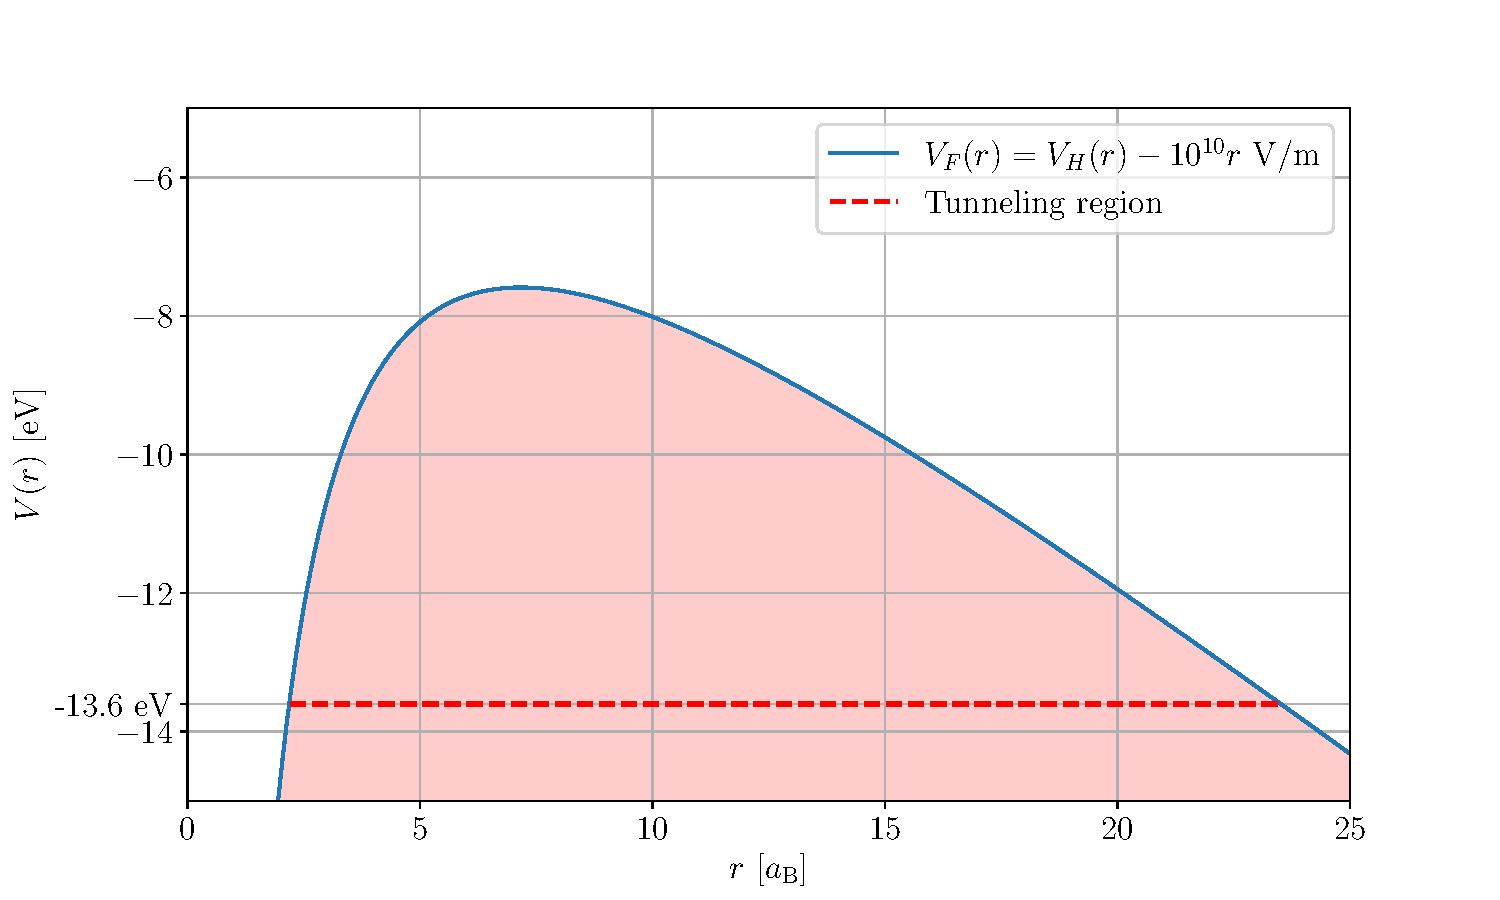
\includegraphics[width=0.8\textwidth]{figures/tunnelling}
	\caption{The potential of hydrogen atom modified by external field: $E_{\mathrm{ext}} = -10^{10}r\,\mathrm{V/m}$. $r$ is shown the radial coordinate normalized to Bohr radius $\mathrm{a_B}$. Energy of ground state of electron in hydrogen atom $E_0 = 13.6\, \mathrm{eV}$ is highlighted.}
	\label{fig:tunnelling}
\end{figure}

The stronger is the external field, the shorter is the tunnelling distance for the electron to escape and the the higher is the probability that this can happen. The field can even be so strong that the potential barrier will have its peak below the ground state energy. In that case, the electron is instantly considered to be free \cite{laser-plasma1}. 

It is possible to estimate, which mechanism is more dominant cause of ionization by calculating so called \textit{Keldysh parameter} $\gamma_\mathrm{K} = \frac{\omega_0}{\omega_t}$, where $\omega_0$ is the frequency of the laser and $\omega_t = \frac{eE_{\mathrm{ext}}}{\sqrt{2mE_\mathrm{i}}}$, where $E_\mathrm{i}$ represents the energy the electron needs to receive to be ionized \cite{laser-plasma1}.

The ionization processes can be explored in greater depth, but the fundamental concepts have already been adequately outlined. Henceforth, we will assume the plasma being targeted by the laser is fully ionized and will focus on how it can absorb additional energy from the laser.

\section{Absorption of ultra-short, ultra-intense lasers}
Modern lasers can generate pulses with durations of only few femtoseconds and extremely high intensities (up to 
$10^{22}\,\mathrm{W.cm}^{-2}$) \cite{absorption2,ultra-laser}. The interaction of such pulses with dense plasma produces hot electrons \cite{laser-plasma5}. There are several processes of energy transfer from the laser's electromagnetic field to the electrons. Let us examine the most significant of these processes.

\subsection*{Collisional absorption}
The principles of collisional absorption are similar to those of collisional ionization. In this process, an electron oscillates due to the influence of the laser field and transfers part of its kinetic energy to other ions through collisions. However, since the frequency of ion-electron collisions scales as $\nu_{ie} \propto E^{-3/2}$, this absorption mechanism is primarily significant for laser intensities below $10^{15}\,\mathrm{W.cm}^{-2}$ \cite{absorption1}. Given that this thesis focuses on intensities above this threshold, further discussion on collisional absorption is unnecessary.

\subsection*{Resonance absorption}
The first non-collisional absorption process we will describe is the \textit{resonance absorption}. This phenomenon can occur during the propagation of a p-polarized light wave through a density gradient. By p-polarized, we refer to a wave that is linearly polarized with its polarization vector lying in the plane of incidence. The complete analytical description is difficult, but after few simplifications it is possible to obtain reasonable idea of the principle \cite{laser-plasma6}. 

Laser light will reach density $n_t = n_{\mathrm{cr}}\cos^2\theta$ (from Snell's law \cite{absorption2}), where $\theta$ is the angle of incidence \cite{laser-plasma6}. At this turning point, some light energy will tunnel through the critical density and the electron plasma will be resonantly excited at frequency of the laser $\omega_0$. The resonant wave is then capable of accelerating electrons and is defined by:
\begin{equation}
	\label{eq:resonance}
	\frac{E_d}{\epsilon} = \frac{E_L}{\sqrt{2\pi\omega_0 L_n/c}}\phi\left(\tau\right)
\end{equation}
where $\epsilon$ is plasma dielectric function, $L_n$ is the density length scale and the parameter $\tau= \left(\omega_0 L_n/c\right)^{1/3}\sin\theta$ and $\phi\left(\tau\right) \propto \exp\left(-2\tau^3/3\right)$ \cite{absorption2,laser-plasma6}.

The angle of optimum resonance absorption for exponential density profile $\theta_{opt}$ can then be estimated as a function of $L$:
\begin{equation}
	\theta_{opt}\left(L\right) = \arcsin\left(0.68(2\pi L)\right)
\end{equation}
where $L$ is normalized to the laser wavelength \cite{absorption1}.


\subsection*{Vacuum heating}
The second non-collisional absorption process (and no less important than the first one) is called \textit{Vacuum heating} or sometimes \textit{Brunel effect} or even \textit{“not-so-resonant” resonance absorption} \cite{brunel1987}. It was proposed by Brunel in 1987 it was later confirmed by many experiments \cite{absorption2}.

Like before, p-polarized laser pulse is needed. At the angle of incidence $\theta$ the laser is hitting the target with steep density profile (a big gradient). A part of the pulse is reflected. The incoming laser wave $\bm{E}_\mathrm{L}$ and reflected wave $\bm{E}_\mathrm{R}$ are in superposition perpendicular to the target surface and the resulting field has a perpendicular component with amplitude $E_0 =  2E_\mathrm{L}\sin\theta$, under approximation that $E_\mathrm{R}=E_\mathrm{L}$. Poisson's equation at the surface gives us \cite{absorption2}:
\begin{equation}
	\label{eq:poisson}
	\Delta E = -4\pi e\int_{x=-\Delta x}^{x=0}n_\mathrm{e} \mathrm{d}x=4\pi e n_\mathrm{e} \Delta x.
\end{equation}
The electrons are pulled out from plasma by the field $E_0$. If $n=N/\left(A\Delta x\right)$ with $N/A$ being number of electrons pulled out into vacuum per unit area $A$ and if $\Delta E = E_0$, we get \cite{absorption2}:
\begin{equation}
	\frac{N}{A} = \frac{2E_0 \sin \theta}{4\pi e}.
\end{equation}
The energy absorbed $E_{\mathrm{abs}}$ by the electrons is then \cite{absorption2}:
\begin{equation}
	E_{\mathrm{abs}} = \frac{1}{2}N m_\mathrm{e} v_{\mathrm{e}}^2.
\end{equation}
After calculating the power absorbed by unit area and after substituting $v_\mathrm{e}$ with \textit{quiver velocity} $v_{osc}$ defined by: $\frac{ v_{osc}}{c} = \frac{eE_0}{m_{\mathrm{e}}c\omega_0}$, we get the absorbed fraction of the power $f_{\mathrm{VH}} = I_{\mathrm{abs}}/I_0$ \cite{absorption2}:
\begin{equation}
	f_{\mathrm{VH}} = 8 \frac{v_{\mathrm{osc}}}{c}sin^3\theta
\end{equation}
Note that we made a simplification by letting $E_\mathrm{R}=E_\mathrm{L}$. Another option would be to directly write $E_0 =  \left(1+R^{1/2}\right)E_\mathrm{L}\sin\theta$, where $R$ is the reflectivity \cite{absorption1}. We also neglected that the electron in vacuum is very fast and therefore relativistic correction has to be made. It is possible to generally follow a more rigorous path found for example in \cite{laser-plasma5} and \cite{absorption1}. Then the formula for $f_{\mathrm{VH}}$ is expanded to:
\begin{equation}
	\label{eq:vac-heating}
	f_{\mathrm{VH}} = \frac{\eta}{2\pi}\frac{1}{a_0}\frac{sin\theta}{cos\theta}\left(1+R^{1/2}\right)\left\{\left[1+\left(1+R^{1/2}\right)^2a_0^2\sin^2\theta\right]^{1/2}-1\right\},
\end{equation}
where $\eta = 1.74$ and $a_0 = eE_\mathrm{L}/(m_\mathrm{e}\omega_0c)$.

\subsection*{$\bm{J}\times \bm{B}$ heating}
The last absorption mechanism we want to discuss is usually called $\bm{J}\times \bm{B}$ \textit{heating}. In the sections above, we discussed the heating of plasma due to electron motion in the direction of the oscillating $\bm{E}$ component of the laser beam. That is of course caused by the $e\bm{E}$ part of the Lorentz force. The other part - $\bm{j \times B}$ - can be neglected in non-relativistic cases. However, for laser intensities higher than $10^{17}\,\mathrm{W.cm}^{-2}$ it is not possible to explain all absorption using the classical limit and another consideration has to be made \cite{cai2006}.

Let $\phi$ and $\bm{A}$ be scalar and vector potential ($\bm{E} = -\nabla \phi -\frac{\partial \bm{A}}{\partial t}$ and $\bm{B} = \nabla \times \bm{A}$) satisfying Coulomb gauge $\nabla \cdot \bm{A} = 0$. Also, we can separate transverse and longitudinal part of electron momentum $\bm{p} = \bm{p}_\mathrm{t}+\bm{p}_\mathrm{l}$  Then the equations of motion for electron can be written as \cite{cai2006}:
\begin{equation}
	\frac{\partial \bm{p}_\mathrm{t}}{\partial t} = \frac{e}{c} \frac{\partial \bm{A}}{\partial t}
	\label{eq:jxb1}
\end{equation}
\begin{equation}
	\frac{\partial \bm{p}_\mathrm{l}}{\partial t} = e\nabla \phi - m_{\mathrm{e}}c^2\nabla (\gamma-1)
	\label{eq:jxb2}
\end{equation}
where $\gamma = \sqrt{1+\frac{a_0^2}{2}}$ is the relativistic factor for linearly polarized light \cite{absorption2}. $a_0$ is the same as defined in equation \ref{eq:vac-heating}, but here is has meaning of a constant normalizing vector field $\bm{A}$. To be more precise $a_0 = \norm{\bm{a}}$ and:
\begin{equation}
	\bm{a} = \frac{e\bm{A}}{m_ec^2}.
\end{equation}

The second term of the equation \ref{eq:jxb2} is the relativistic ponderomotive force and we can write the ponderomotive potential $U_\mathrm{p}$ as:
\begin{equation}
	U_\mathrm{p} = (\gamma - 1)m_{\mathrm{e}}c^2.
	\label{eq:ponderomotive-potential}
\end{equation}
There is a force with frequency $2\omega_0$ which will affect the electrons in longitudinal direction. One of the interpretations of this force can sound like this: Twice every laser period, streams of electrons are pushed into the the target \cite{cai2006}. This causes the production of fast electrons.

It is important to note, that at higher intensity, the electron density can rise as a consequence of the zero-frequency pondermotive force. The change in density can cause the $2\omega_0$ force component to be inefficient for hot electron generation. The density is also related the scale length of the target. For example for exponential density profile, the density decreases with the increase of scale length \cite{cai2006}. This means the $\bm{J}\times \bm{B}$ heating is expected to play a greater role for bigger scale lengths. In other words, the initial plasma conditions need to be known to estimate the effects of $\bm{J}\times \bm{B}$ heating.

One last note regarding $\bm{J}\times \bm{B}$ heating. The relativistic factor $\gamma$ has a different form in a case of circularly polarized laser. That leads to suppressing this kind of electron heating altogether \cite{cai2006}.


The three mentioned mechanisms are by no means exhaustive when it comes to laser absorption. They are the three most relevant in the context of this work. There are other physical processes contributing to heating up the plasma especially when the parameters of the experiment change \cite{absorption1}. We will now move on to describe the particular motivation of the thesis.

\section{Motivation - X-ray $\mathbf{K}_\alpha$ emission}
Because hot electrons accelerated by ultra-intense ultra-short laser pulse can carry significant (keV-MeV) energy, they can penetrate deeper into the unionized part of the target, where they can generate characteristic X-rays by K-shell ionization \cite{reich2000}. The X-ray spectrum is consisting of spectral lines (e.g. $\mathrm{K}_\alpha$) and continuous part X-ray from Bremsstrahlung. The uniqueness of this method of producing X-rays rests in the monochromatic spectrum of high energy X-ray photons within a short pulse synchronized with the laser pulse. The source is typically very small \cite{pfeifer2006}.

\begin{figure}[h]
	\centering
	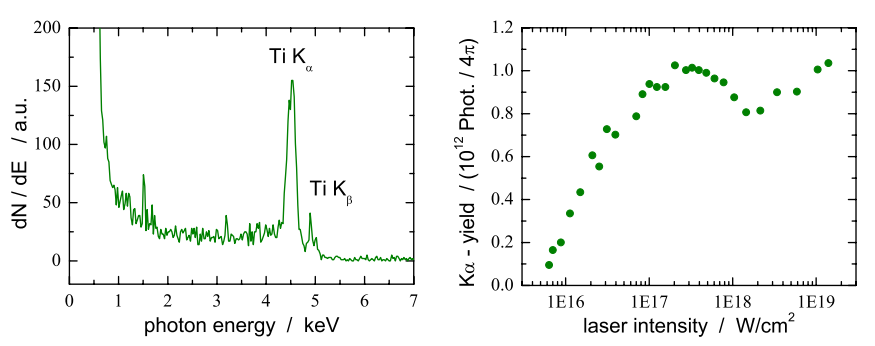
\includegraphics[width=0.95\textwidth]{figures/spectrum-ti}
	\caption{\textit{Left:} The spectrum of laser generated $\mathrm{K}_\alpha$ and $\mathrm{K}_\beta$ radiation of titanium. \textit{Right:} The scaling of $\mathrm{K}_\alpha$ - yield in relation to laser intensity. \cite{schwoerer2004}}
	\label{fig:ti-spectrum}
\end{figure}

Let us now briefly look into the origin $\mathrm{K}_\alpha$-line. In figure \ref{fig:ti-spectrum}, there is an energy spectrum of titanium x-ray photons and the $\mathrm{K}_\alpha$ - yield scaling with the laser intensity. The generation of the $\mathrm{K}_\alpha$ radiation clearly depends on laser intensity through the hot electrons temperature. According to \cite{schwoerer2004}, the yield drops at the laser intensity around $10^{18}\,\mathrm{W.cm}^{-2}$ \textit{"because the interaction time with the atom decreases with higher electron velocity"}. The following rise in the yield is then attributed to the relativistic effect where the electric fields of the fast hot electrons are contracted and therefore have greater effect \cite{schwoerer2004}.

The total yield $N$ can be expressed analytically as \cite{reich2000}:
\begin{equation}
	N_{\mathrm{yield}} = \int n_\mathrm{hot} f_\mathrm{hot}(E) N_\mathrm{gen}(E) f_\mathrm{em}(E)\mathrm{d}E
	\label{eq:total-yield}
\end{equation}
where $N$ is the number of emitted photons, $n_\mathrm{hot}$ is the total number of hot electrons, and $f_\mathrm{hot}(E)$ is their energy distribution, $N_\mathrm{gen}(E)$ is the number of $\mathrm{K}_\alpha$ photons generated by an electron of incidence energy E, and $f_\mathrm{em}(E)$ is the fraction of these photons that escapes from the solid \cite{reich2000}. 

Having a reliable numerical model for $n_\mathrm{hot}$ and $f_\mathrm{hot}(E)$ from equation \ref{eq:total-yield} based on the parameters of the laser and the plasma could allow us to optimize the $\mathrm{K}_\alpha$ yield. Namely, the angle of incidence, the laser intensity and the plasma length scale are the most important parameters for laser absorption. The research conducted by Reich et al. \cite{reich2000} could be followed up by examining a wider range of parameters beyond just laser intensity. This is crucial because, as shown by Cui et al. \cite{cui2013}, the temperature function of the electrons has a complex and non-trivial shape. The complexity comes from the complex nature of the physical processes causing the electron heating.

In this thesis, we presents results from hundreds of PIC simulations while scanning through the mentioned parameters. Then we try to present and  defend a way of how the hot electron temperature can be modelled and how to make the model more precise. The implications with respect to previous works and to equation \ref{eq:total-yield} are discussed.

\section{PIC simulations}
As previously mentioned, we are using Particle-In-Cell (PIC) simulations to obtain the data necessary for our model. PIC codes have been under development since the advent of computers in the 1960s, and advancements in computer technology over the past 30 years have enabled us to run simulations on a much larger scale. One significant advantage of simulations is that they allow theoretical predictions to be verified in greater detail than is possible with real plasma experiments \cite{dawson1962}. To illustrate the progress made over the decades, let us mention, that in 1962 Dawson and Buneman simulated the motion of $1000$ plasma particles. Today, we can simulate the motion of more than $10^{10}$ particles \cite{tskhakaya2007}.

We are not developing our own simulation code. Instead, we are using code freely available for academic purposes, specifically the 2D version of simulation code EPOCH \cite{arber2015}. EPOCH has been widely used in numerous publications within the laser-plasma field and adequately meets our requirements. Below, we will present a brief overview of the key principles of the PIC method, upon which EPOCH is also based.

\subsection*{Macro-particles}
It is not possible to have as many particles in a simulation as in a real plasma, even in very small scales, because of the computational cost. Because of that, the simulations usually work with macro-particles which represent clouds of many real particles. These particles have finite sizes (as opposed to infinitesimal), so that there are no divergent forces in case of collisions. The forces in simulations go to zero for small distances between macro-particles. For large distances, they comply with the Coulombic behaviour. In plasma simulations, it is possible to do this without sacrificing accuracy, because of the collective behaviour of plasma\cite{fonseca2009}.

\subsection*{Computational cycle}
The simulation runs in a cycle. In each step, we solve for electromagnetic fields created by the charged particles. Then we evaluate the equations of motion for the particles, which are influenced by the Lorentz force \cite{birdsall1985}. The laser pulse is included as an external source of electromagnetic radiation at the boundary.

Typically, the finite-difference time-domain method (FDTD) is used for numerically solving Maxwell's equations, which fully describe the electromagnetic field. \textit{Finite-difference} means that the electric field $\bm{E}$ and magnetic field $\bm{B}$ are specified in the points of a grid - usually a \textit{Yee grid}. A comprehensive description of a Yee grid can be found in the original article by Yee \cite{yee1966}. The critical concept of a Yee grid is illustrated in figure \ref{fig:yee-grid}. - the magnetic field components are calculated in the center of the faces of an imaginary cube (cell) while the electric field components are calculated in the center of the edges. The cube represents one cell of the 3-dimensional grid. We can approximate derivatives of electric field with centered finite differences \cite{arber2015}:
\begin{equation}
	\label{eq:num-der}
	\left(\frac{\partial E_y}{\partial x}\right)_{i+\frac{1}{2},j,k} = \frac{E_{y,i+1,j,k}-E_{y,i,j,k}}{\Delta x} 
\end{equation}

Note, that this approximation is second order accurate at the cube point where we calculate $B_{z,i,j,k}$, because the formula is centered. Moreover, because of one of the Maxwell's equations, $\nabla \times \bm{E} = \frac{\partial \bm{B}}{\partial t}$, this derivative is exclusively used to calculate time-derivative of $B_{z,i,j,k}$. A similar relationship can be found when calculating all components of $\bm{B}$ from $\bm{E}$ and vice versa. Therefore, all used numerical derivatives are second order accurate \cite{arber2015}.

\begin{figure}[t]
	\centering
	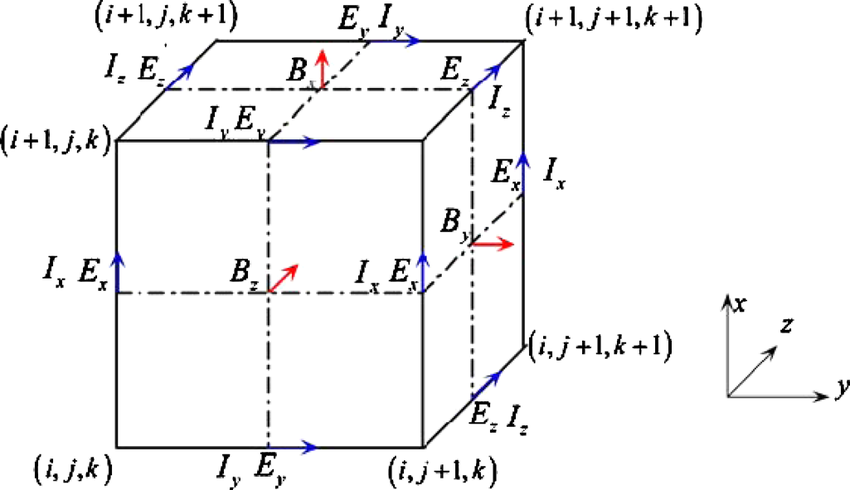
\includegraphics[width=0.6\textwidth]{figures/yee-grid}
	\caption{An illustration of a Yee grid \cite{wang2010}}.
	\label{fig:yee-grid}
\end{figure}

In EPOCH, as in other PIC codes, fields are updated at both the half time-step and full time-step. The first part - time-step from $n$ to $n+1/2$ - uses currents calculated at $n$:
\begin{equation}
	\bm{E}^{n+1/2} = \bm{E}^n + \frac{\Delta t}{2}\left(c^2 \nabla\times\bm{B}^n - \frac{\bm{J}^n}{\epsilon_0}\right)
\end{equation}
\begin{equation} 
	\bm{B}^{n+1/2} = \bm{B}^n - \frac{\Delta t}{2}\left(\nabla\times\bm{E}^{n+1/2} \right)
\end{equation}
where $\bm{J}$ is the current density and $\Delta t$ is a size of a full time-step \cite{arber2015}.

In the second step, we use the updated currents at $n+1$:
\begin{equation} 
	\bm{B}^{n+1} = \bm{B}^{n+1/2} - \frac{\Delta t}{2}\left(\nabla\times\bm{E}^{n+1/2} \right)
\end{equation}
\begin{equation}
	\bm{E}^{n+1} = \bm{E}^{n+1/2} + \frac{\Delta t}{2}\left(c^2 \nabla\times\bm{B}^{n+1} - \frac{\bm{J}^{n+1}}{\epsilon_0}\right)
\end{equation}

The motion of particles and the resulting currents are consequences of the fields. Generally, the equations of motion are:
\begin{equation}
	\frac{\mathrm{d}\bm{x_l}}{\mathrm{d}t} = \bm{v_l} \text{   and   }  \frac{\mathrm{d}\bm{p_l}}{\mathrm{d}t} = \bm{F_l}
\end{equation}
where vectors $\bm{x_l}$,  $\bm{v_l}$  and $\bm{p_l}$ represent the position, velocity and momentum of the \textit{l}-th macro-particle. $\bm{F_l}=\bm{F_l}(t,\bm{x_l},\bm{v_l},\bm{E},\bm{B})$ is the force. Fields $\bm{E}$ and $\bm{B}$ are functions of the positions and time \cite{tskhakaya2007}.
In this context, the right-hand side of the second equation represents the Lorentz force, and the time-step formula for the momentum is: \cite{arber2015}:
\begin{equation}
	\bm{p}^{~n+1}_{l} = \bm{p}^{~n}_l + q_l\Delta t \left[\bm{E}^{n+1/2}\left(\bm{x}_l^{~n+1/2}\right)+\bm{v_l}^{n+1/2}\times \bm{B}^{n+1/2}\left(\bm{x}_l^{~n+1/2}\right) \right] 
	\label{eq:mom-up}
\end{equation}
where $q_l$ is the charge of the $l$-th particle. The velocity can be calculated from the momentum using:
\begin{equation}
	\bm{v}_l = \frac{\bm{p}_l}{\gamma_l m_l}
\end{equation}
where $m_l$ is the mass of the particle and $\gamma_l = [p_l^2/(m_l^2 c^2)+1]^{1/2}$ is the corresponding gamma-factor \cite{arber2015}.

The particle position update is calculated from the velocity, but this is also done in multiple steps. First, we calculate movement of half time-step from the old velocity as we need it to update the momentum in equation \ref{eq:mom-up} \cite{arber2015}:
\begin{equation}
	\bm{x}^{~n+1/2}_{l} = \bm{x}^{~n}_l + \frac{\Delta t}{2} \bm{v}^{~n}_l  
\end{equation}
In similar way, we can then calculate $\bm{x}^{~n+1}_l$ and $\bm{x}^{~n+3/2}_l$ \cite{arber2015}, which are needed for calculating the currents.

The currents necessary for updating the fields can be calculated using methods such as the one presented by Esirkepov in \cite{esirkepov2001}. Modern approaches to calculating currents are generally based on solving the discrete form of the continuity equation:
\begin{equation}
	\frac{\partial\rho}{\partial t} + \nabla \cdot \bm{J} = 0
	\label{eq:conti}
\end{equation} 
where $\rho$ is the charge density and $\bm{J}$ is the electric current. This can be discretized as:
\begin{equation}
	\frac{\rho^{n+1}_{i+1/2,j+1/2,k+1/2}-\rho^{n}_{i+1/2,j+1/2,k+1/2}}{\Delta t} + \frac{J^{n+1/2}_{x,i+1,j+1/2,k+1/2}-J^{n+1/2}_{x,i,j+1/2,k+1/2}}{\Delta x} + \dots = 0.
\end{equation}

The charge density is calculated using \textit{form-factors} of macro-particles:

\begin{equation}
	\rho_{i,j,k} = \sum_{l}Q_l S_{i,j,k}(x_l,y_l,z_l)
\end{equation}
where $Q_l$ is the charge and $S_{i,j,k}(x_l,y_l,z_l)$ is the form-factor. During macro-particle motion, the total charge should remain constant, necessitating that the form-factors satisfy the condition :
\begin{equation}
	\sum_{i,j,k}S_{i,j,k}(x_l,y_l,z_l) = 1
\end{equation}
Since macro-particles in the simulation represent numerous real particles, a \textit{weight} is assigned to each macro-particle. Although the exact particle distribution within a macro-particle is unknown, a representative function, known as a \textit{shape function}, is chosen.\cite{arber2015}. 

Any function with a unit integral and compact support can be used as a shape function. An even distribution of particle in volume $\Delta x \times \Delta y \times \Delta z$ is referred to as the \textit{top hat} shape function. Using higher order shape functions are one of the improvements programmers were able to make thanks to more powerful computers. A higher order shape functions are for example triangular shape functions with volume of $2\Delta x \times 2\Delta y \times 2\Delta z$  . The weight is then calculated as a convolution of shape function with the 'top hat' function \cite{arber2015}.

Working with macro-particles instead of individual particles neglects some effects, particularly those effective over distances shorter than $\Delta x$. EPOCH uses a fully relativistic, energy-conserving binary collision model, which favors small-angle scattering to improve simulation behavior with a limited number of particles per cell. For our study involving laser intensities above $10^{10}$, collisions are not necessary. Other effects, such as ionization and quantum phenomena like photon emission and pair production, are often included when relevant, with detailed descriptions available in~\cite{arber2015}.
\chapter{Temperature fitting}
\label{ch:temp-fitting-theory}
The results of the EPOCH simulations provide weighted momenta for a subset electrons $\bm{p}_\mathrm{e}$, where the weight represents the number of electrons with that momentum. They are not histograms yet, because more than one macro-particle can have the same value of $\bm{p}_\mathrm{e}$. The energies of electrons can then be calculated from $\bm{p_\mathrm{e}}$ using the relativistic formula:
\begin{equation}
	\label{eq:rel-energy}
	E_\mathrm{e} = m_\mathrm{e}\cdot c^2\left(\sqrt{1+\left(\frac{p_\mathrm{e}}{m_\mathrm{e}\cdot c}\right)^2} -1\right)\mathrm{,}
\end{equation}
where $p_\mathrm{e}=\sqrt{\bm{p}_\mathrm{e}\cdot\bm{p}_\mathrm{e}}$ is the size of $\bm{p}_\mathrm{e}$, $m_\mathrm{e} =  9.109 \times 10^{-31} \, \mathrm{kg}$ is the electron rest-mass and $c=3\times 10^{8} \, \mathrm{m . s}^{-1}$ is the speed of light \cite{mohr2016}.

\begin{figure}[h]
	\centering
	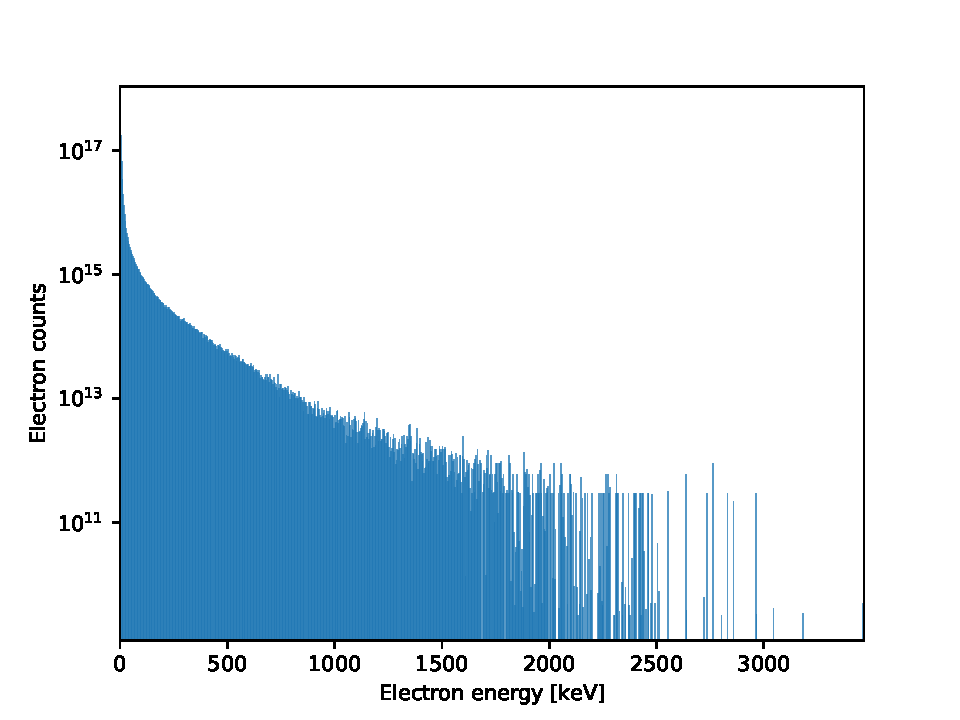
\includegraphics[width=0.7\textwidth]{figures/example-histogram}
	\caption{An example of electron energy distribution of 2D EPOCH simulation with intensity of laser $I=10^{19}\,\mathrm{W.cm}^{-2}$, characteristic scale of the exponential preplasma profile $L=0.1\,\mathrm{\mu m}$ and angle of incidence with respect to target normal direction $\alpha = 10$°.}
	\label{fig:example-histogram}
\end{figure}
One can easily create the histogram from electron energies and their counts. An example of such histogram can be seen in the figure \ref{fig:example-histogram}. There are several things that need to be discussed.

Firstly, it is important to note that the $y$-axis is presented on a logarithmic scale to enhance readability. The extensive range of electron energies necessitates the use of relativistic formula. However, around the energies $E_k \approx 1900 \, \mathrm{keV}$ and more, the histogram exhibits irregularities - specifically, there are empty bins and several bins contain identical electron counts. These anomalies are attributed to the resolution of the simulation. Consequently, this portion of the spectrum is rendered questionable. This issue will be further addressed in the section dedicated to temperature fitting.

Last but not least, note the apparent exponential relationship between $N_i$ and $E_k$ in the energy spectrum between $E_k \approx 500 \, \mathrm{keV}$ and $E_k \approx 1500 \, \mathrm{keV}$:
\begin{equation}
	\label{eq:exp-distr}
	N_i = N_0 \cdot \mathrm{exp}\left( -\frac{E_i}{T}\right)\mathrm{,}
\end{equation}
where $N_i$ is count in $i$-th bin and $E_i$ is the corresponding energy and $T$ is temperature in units discussed in section \ref{sec:temperature-intro}. The relationship is, of course, linear after the logarithmic transformation. The equation of \ref{eq:exp-distr} resembles exponential distribution with $1/T$ missing on the right-hand side. It is also not normalized, because it represents counts that have to add up to total number of electrons with that temperature. For the purpose of this thesis, we will call it the \textit{Boltzmann distribution}, even though it is not completely accurate.

Fitting the correct part of the histogram using equation \ref{eq:exp-distr} and estimating $T$ and $N_0$ is the first bigger part of this thesis. There are several obstacles, all of which are discussed in following sections.

\section{Boltzmann vs. Maxwellian distribution}
First of all, in section \ref{sec:temperature-intro}, where we introduced temperature as a quantity describing plasma, we said that the distribution of energies is usually considered to be Maxwellian. The question, whether we can fit our histogram using Boltzmann distribution, is therefore valid and needs to be addressed.

The equations for the Maxwellian $f_\mathrm{M}(E)$ and Boltzmann $f_\mathrm{B}(E)$ distributions can be after few simplifications regarding units defined as:
\begin{equation}
	f_\mathrm{M}(E)\mathrm{d}E = \frac{\sqrt{E}}{(T)^{3/2}}\exp\left(-\frac{E}{T}\right)\mathrm{d}E
\end{equation}
and
\begin{equation}
	f_\mathrm{B}(E)\mathrm{d}E = \frac{1}{T}\exp\left(-\frac{E}{T}\right)\mathrm{d}E.
\end{equation}
By ignoring that both are defined by the differential, taking logarithm of both $f_\mathrm{M}(E)$ and $f_\mathrm{B}(E)$ we get:
\begin{equation}
	\bar{f_\mathrm{M}}(E) = \ln\left(f_\mathrm{M}(E)\right) = \ln\left(\frac{\sqrt{E}}{(T)^{3/2}}\right)+\left(-\frac{E}{T}\right)
\end{equation}
and
\begin{equation}
	\bar{f_\mathrm{B}}(E) = \ln\left(f_\mathrm{B}(E)\right) = \ln\left(\frac{1}{T}\right)+\left(-\frac{E}{T}\right).
\end{equation}
These two equations describe the the distributions in a logarithmic scale. The first derivatives are then:
\begin{equation}
	\label{eq:slope-maxwell-log}
	\frac{\mathrm{d}\bar{f_\mathrm{M}}}{dE} =-\frac{1}{2}\frac{T^{3/2}}{\sqrt{E}}\frac{1}{T^{3/2}\sqrt{E}}-\frac{1}{T} = -\frac{1}{2E}-\frac{1}{T}
\end{equation}
and
\begin{equation}
	\label{eq:slope-boltzmann-log}
	\frac{\bar{f_\mathrm{B}}}{dE} = -\frac{1}{T}.
\end{equation}
The equations \ref{eq:slope-maxwell-log} and \ref{eq:slope-boltzmann-log} suggest that, in the logarithmic scale, the slopes of these distributions differ by $-\frac{1}{2E}$, which decreases with increasing $E$. In other words, the fit of $T$ can be replaced by fitting slope $s = -1/T$ of the histogram after logarithmic transformation. For large energies, the slopes of both discussed distributions are approximately equal. 

Moreover, the assumption of Boltzmann distribution allows us to fit not only the temperature, but also $N_0$, which is the total number of electrons in that distribution of hot electrons. If we keep the form of the distribution as in equation \ref{eq:exp-distr}, the total energy absorbed by the group of hot electrons $E_{\mathrm{tothot}}$ with temperature $T_\mathrm{hot}$ can be calculated as:
\begin{equation}
	E_{\mathrm{tothot}} = N_0\cdot T_\mathrm{hot}.
\end{equation}


\section{Exponential-sum fitting}
\label{sec:exp-fit}
Exponential-sum fitting has been a recognized challenge for many years. Forman S. Acton, a professor at Princeton University, addressed this issue in his 1970 book Numerical Methods That Work. Among various topics, he included an essay titled "What Not to Compute," wherein he described the fitting of sums of exponential functions as "extremely ill-conditioned"~\cite{acton1990}. Despite the inherent difficulty of this problem, this thesis endeavors to determine electron temperatures, necessitating the development of an effective solution to this challenging computational task. 

The task is to find the parameters $m, a_0, a_1,..., a_m, b_1,...b_m$ so that the function

\begin{equation}
	f(x) = a_0 + \sum_{i=1}^{m} a_i \mathrm{e}^{b_i x}
\end{equation}

generalizes the data as good as possible. Formally, for a set of data ($n$ data points) $\left(\left(x_1,y_1\right),..., \left(x_n,y_n\right)\right)$ we are minimizing error function

\begin{equation}
	e = \sum_{i=1}^{n}w_i(y_i-f(x_i))^2
\end{equation}

where $w_i$ are the weights.

Modern programming libraries provide access to well-known and generally efficient methods, such as non-linear least squares. However, due to the previously mentioned ill-conditioning, these methods do not yield satisfactory results in this context. The convergence of these methods is highly dependent on the quality of the initial guess, which poses a significant challenge. To date, significant efforts have been made to develop reliable methods for solving this problem. 

Notably, Prony's method \cite{prony1795} and its variations, as discussed in sources such as \cite{potts2010}, have been proposed. It was originally intended for signal approximation - specifically, the determination of complex parameters in exponential functions, similar to Fourier transformation.

Another, much simpler method is known as \textit{successive subtraction}~\cite{wiscombe1977}. This method is frequently employed for exponential decays (negative parameters $b_i$), which closely resemble our problem of exponential distributions. The core concept involves fitting the end of the decay with a single exponential function, subtracting this result from the data, and iteratively identifying all exponential components. This simplicity makes it a promising candidate for our problem, especially since our primary interest lies in determining the temperature of the hottest electrons—the tail. However, automating this method can be challenging, as it is not straightforward to select an interval that can be fitted as a tail in each iteration. Moreover, the tail of our histograms are not reliable as was discussed with regard of the example histogram in figure \ref{fig:example-histogram}.

Another method worth considering is presented in \cite{wiscombe1977}. This method, called exponential sum fitting of transmissions (ESFT), was developed for fitting radiative transmission functions in the context of atmospheric research. ESFT too is an iterative method and might serve as an interesting alternative for future works.

We only mentioned a few methods. A summary with a deeper explanation of these and other methods can be found in \cite{wiscombe1977}, \cite{holmstrom2002} or in \cite{hokanson2013}.

If the goal is to fit only one of the exponentials, such as the parameters of the hot electrons distribution, the standard approach involves manually selecting the "correct" segment of the distribution and fitting it with a single exponential function. For instance, in \cite{cui2013}, where researchers study a problem similar to ours, they appear to use this technique to determine the temperature of hot electrons. The term "correct" is somewhat vague because it can be subjective and we do not have any metric that would quantify how well the segment was chosen. We can only work with the metrics describing the fit itself.

The last mentioned option currently provides the most reliable approach to fitting the temperature of hot electrons. Even for hundreds of simulations, with the right tool, it is possible to fit manually every histogram within few hours. Having such dataset of histograms and temperatures is valuable for evaluating any method that is trying to automate the fitting process. A tool with an UI was developed specifically for this purpose as a part of this work.

That being said, we still attempted to automate the fitting. The method we used is explicit an non-iterative.

\subsection*{The 'Jacquelin' method}
\label{sec:jaquelin}
We will call the method we chose \textit{Jacquelin method}, because we will be referencing an article by J.Jacquelin who developed it for his own purpose \cite{jacquelin2014}. This method is explicit and non-iterative which is its main advantage. The original derivation presents a universal strategy how to explicitly approximate any function that is a solution to some integral or differential equation. Let us start with derivation of the numerical algorithm for a function:

\begin{equation}
	\label{eq:orig-eq}
	y(x) = a_0 + a_1\mathrm{e}^{b_1x} + a_2\mathrm{e}^{b_2x}
\end{equation}
We start by calculating these integrals:
\begin{flalign*}
	\;\;\;\;\;\;\;\;\;\;\;\; S(x) & = \int_{x_0}^{x}y(t) \mathrm{d}t \\
	& = \int_{x_0}^{x}a_0 + a_1\mathrm{e}^{b_1t} + a_2\mathrm{e}^{b_2t} \mathrm{d}t \\
	& = a_0(x-x_0) + \frac{a_1}{b_1}(\mathrm{e}^{b_1x}-\mathrm{e}^{b_1x_0}) +
	\frac{a_2}{b_2}(\mathrm{e}^{b_2x}-\mathrm{e}^{b_2x_0}) &
\end{flalign*}

\begin{flalign*}
	\;\;\;\;\;\;\;\;\;\;\;\; SS(x) & = \int_{x_0}^x S(t)\mathrm{d}t \\
	& = \int_{x_0}^x\int_{x_0}^{t}y(u) \mathrm{d}u\mathrm{d}t \\
	& = \int_{x_0}^{x}a_0t + \frac{a_1}{b_1}\mathrm{e}^{b_1t} +
	\frac{a_2}{b_2}\mathrm{e}^{b_2t} - \left(\frac{a_1}{b_1}\mathrm{e}^{a_1 x_0}+\frac{a_2}{b_2}\mathrm{e}^{a_2 x_0}+a_0x_0\right)\mathrm{d}t \\
	& = \frac{1}{2}a_0x^2 - \left(\frac{a_1}{b_1}\mathrm{e}^{a_1 x_0}+\frac{a_2}{b_2}\mathrm{e}^{a_2 x_0}+a_0x_0\right)(x-x_0) -\frac{1}{2}a_0x_0^2 \\ 
	& \;\;\; + \frac{a_1}{b_1^2}\left(\mathrm{e}^{b_1x} - \mathrm{e}^{b_1x_0}\right)  + \frac{a_2}{b_2^2}\left(\mathrm{e}^{b_2x} - \mathrm{e}^{b_2x_0}\right) &&
\end{flalign*}

Now, if we reorganize the terms it can be shown that there are constants $A$, $B$, $C$, $D$ and $E$ so that $y(x)$ can be written as:
\begin{equation}
	\label{eq:lin}
	y(x) = A\cdot SS(x)+B\cdot S(x) + C x^2 + Dx + E.
\end{equation}
By comparing coefficients before the exponential terms $\mathrm{e}^{b_1 x}$ and $\mathrm{e}^{b_2 x}$ we get:
\begin{align}
	a_1 & = A\frac{a_1}{b_1^2} + B\frac{a_1}{b_1}  \\
	a_2 & = A\frac{a_2}{b_2^2} + B\frac{a_2}{b_2}
\end{align}
From that it is possible to see that $b_1$ and $b_2$ are roots of the quadratic equation:
\begin{equation}
	\label{eq:quadratic}
	b^2 - bB - A = 0.
\end{equation}
$b_1$ and $b_2$ are then:
\begin{align}
	\label{eq:roots}
	b_1 = & \frac{1}{2}\left(B + \sqrt{B^2 + 4A}\right) \\
	b_2 = & \frac{1}{2}\left(B - \sqrt{B^2 + 4A}\right)
\end{align}

The equation \ref{eq:lin} is linear in the unknown parameters $A,..,E$ and after discretization it can be rewritten as: 
\begin{equation}
	\label{eq:lin-vec}
	\boldsymbol{y}=\boldsymbol{X}\cdot \boldsymbol{b}
\end{equation}
where $\boldsymbol{y}$ is vector:
\begin{equation}
	\boldsymbol{y} =
	\begin{pmatrix}
		y_1 \\
		y_2 \\
		\vdots \\
		y_n  
	\end{pmatrix}
\end{equation} 	

Denoting $S_k=S(x_k)$ and $SS_k=SS(x_k)$ we can write:
\begin{equation}
	\boldsymbol{X} =
	\begin{pmatrix}
		SS_1 & S_1 & x_1^2 & x_1 & 1 \\
		SS_2 & S_2 & x_2^2 & x_2 & 1 \\
		SS_3 & S_3 & x_3^2 & x_3 & 1 \\
		\vdots & \vdots & \vdots & \vdots & \vdots \\
		SS_n & S_n & x_n^2 & x_n & 1  
	\end{pmatrix}
\end{equation}
and 
\begin{equation}
	\boldsymbol{b} =
	\begin{pmatrix}
		A \\
		B \\
		C \\
		D \\
		E  
	\end{pmatrix}.
\end{equation}

We can use the well-known least squares method to calculate the parameters $A,...,E$. We sort the data so that if $i<j$, then $x_i<x_j$ for $\forall i,j \in \{1,..,n\}$. The integrals are computed numerically as:
\begin{equation}
	S_i = \left\{
	\begin{array}{ll}
		0 & i=0 \\
		S_{i-1} + \frac{1}{2}(y_i+y_{i-1})(x_i-x_{i-1}) & i\in\{2,...n\}
	\end{array}
	\right.
\end{equation}
and
\begin{equation}
	SS_i = \left\{
	\begin{array}{ll}
		0 & i=0 \\
		SS_{i-1} + \frac{1}{2}(S_i+S_{i-1})(x_i-x_{i-1}) & i\in\{2,...n\}
	\end{array}
	\right.
\end{equation}

Now, the solution to the linear equation \ref{eq:lin-vec} can be written as \cite{lin-reg}:

\begin{equation}
	\boldsymbol{b}=\left(\boldsymbol{X}^T\boldsymbol{X}\right)^{-1}\cdot (\boldsymbol{X}^T\boldsymbol{y})
\end{equation}
which in our case can be expanded to:

\begin{equation}
	\label{eq:lin-reg}
	\begin{pmatrix}
		A \\
		B \\
		C \\
		D \\
		E  
	\end{pmatrix} 
	=
	\begin{pmatrix}
		\sum\limits_{i=1}^nSS_i^2 & \sum\limits_{i=1}^nSS_iS_i & \sum\limits_{i=1}^nSS_ix_i^2 & \sum\limits_{i=1}^nSS_ix_i & \sum\limits_{i=1}^nSS_i \\
		\sum\limits_{i=1}^nSS_iS_i & \sum\limits_{i=1}^nS_i^2 & \sum\limits_{i=1}^nS_ix_i^2 & \sum\limits_{i=1}^nS_ix_i & \sum\limits_{i=1}^nS_i \\
		\sum\limits_{i=1}^nSS_ix_i^2 & \sum\limits_{i=1}^nS_ix_i^2 & \sum\limits_{i=1}^nx_i^4 & \sum\limits_{i=1}^nx_i^3 & \sum\limits_{i=1}^nx_i^2 \\
		\sum\limits_{i=1}^nSS_ix_i & \sum\limits_{i=1}^nS_ix_i & \sum\limits_{i=1}^nx_i^3 & \sum\limits_{i=1}^nx_i^2 & \sum\limits_{i=1}^nx_i \\
		\sum\limits_{i=1}^nSS_i & \sum\limits_{i=1}^nS_i & \sum\limits_{i=1}^nx_i^2 & \sum\limits_{i=1}^nx_i & n  
	\end{pmatrix}^{-1}
	\begin{pmatrix}
		\sum\limits_{i=1}^nSS_iy_i \\
		\sum\limits_{i=1}^nS_iy_i \\
		\sum\limits_{i=1}^nx_i^2y_i \\
		\sum\limits_{i=1}^nx_iy_i \\
		\sum\limits_{i=1}^ny_i  
	\end{pmatrix}
\end{equation}

After we compute $b_1$ and $b_2$ from $\boldsymbol{b}$, we still have 3 unknown parameters $a_0$, $a_1$ and $a_2$. For those, we will take the original equation \ref{eq:orig-eq}. As it is already linear in the parameters $a_0$, $a_1$ and $a_2$, we only need to pre-compute the values of $\alpha_k=\mathrm{e}^{b_1x_k}$ and $\beta_k =\mathrm{e}^{b_2x_k}$.
One can see that we get a very similar equation as \ref{eq:lin-reg}, that can be written in this form:
\begin{equation}
	\begin{pmatrix}
		a_0 \\
		a_1 \\
		a_2
	\end{pmatrix} 
	=
	\begin{pmatrix}
		n & \sum\limits_{i=1}^n\alpha_i & \sum\limits_{i=1}^n\beta_i  \\
		\sum\limits_{i=1}^n\alpha_i & \sum\limits_{i=1}^n\alpha_i^2 & \sum\limits_{i=1}^n\alpha_i\beta_i  \\
		\sum\limits_{i=1}^n\beta_i & \sum\limits_{i=1}^n\alpha_i\beta_i & \sum\limits_{i=1}^n\beta_i^2
	\end{pmatrix}^{-1}
	\begin{pmatrix}
		\sum\limits_{i=1}^ny_i \\
		\sum\limits_{i=1}^n\alpha_iy_i \\
		\sum\limits_{i=1}^n\beta_iy_i
	\end{pmatrix}
\end{equation}

In \cite{jacquelin2014}, only the case without the constant $a_0$ is presented, but as we have shown the derivation of the generalized version with constant is not difficult. An extension of Jacquelin method for more than two exponential terms is also not very complicated. Note that adding one term adds two parameters, which leads to matrix of size $7\times7$. However, it always leads to solving for the roots of the polynomial created by the first $N$ elements of the vector $\boldsymbol{b}$, where $N$ is the number of exponential terms. In case of two exponential terms, equations \ref{eq:roots} solve for the roots of the polynomial of Equation \ref{eq:quadratic}. In case of three exponential terms, we would need to calculate $SSS(x)$ from $SS(x)$. There would also be a term $x^3$. If we set $\boldsymbol{X}$ as $\left[SSS(x),SS(x),S(x),x^3,x^2,x^1,1\right]$, we would solve for the roots of:
\begin{equation}
	b^3-Cb^2-Bb-A=0.
\end{equation}

It is necessary to note, that this algorithm is prone to numerical defects coming from the fact that there is a cumulative error related to the calculation of the partial sums. For that reason the resulting matrices can be singular or the polynomial can have imaginary roots.

In \cite{mokhomo2021}, Mokhomo et al. did numerical experiments where they have shown that similar method (derived from differential instead of integral equations) can be used for fitting, but does not yield precise estimation results even for noiseless data. Nevertheless, it is an explicit algorithm for approximation of parameters which then can be used as initial guess for more advanced iterative techniques.

When it comes to uncertainty of the coefficients, there are two possibilities. First, it is possible to propagate the experimental error from $y_i$ all the way to the final coefficients. The derivation can be found in \cite{lecca2021}. However, we do not have the standard error of the histogram bins. In principle, this can be obtained by repeating the simulation with the same input parameters but with a different seed for the random number generator which provides initial velocities for particles based on Maxwellian distribution. 

The second option is to take the formula for linear regression and calculate the error estimation directly from that from that. In that case, we calculate estimates $\Delta A$ and $\Delta B$ as standard deviations for $A$ and $B$. Then, using the error propagation formula for the quadratic roots we get:
\begin{equation}
	\label{eq:b-coef-error1}
	\Delta b_1 = \sqrt{\frac{\Delta A^2}{(B^2 + 4A)} + \frac{\Delta B^2}{4} \left(1 + \frac{B}{\sqrt{B^2 + 4A}}\right)^2}
\end{equation}
and
\begin{equation}
	\label{eq:b-coef-error2}
	\Delta b_2 = \sqrt{\frac{\Delta A^2}{(B^2 + 4A)} + \frac{\Delta B^2}{4} \left(1 - \frac{B}{\sqrt{B^2 + 4A}}\right)^2},
\end{equation}
where $\Delta b_1$ and $\Delta b_2$ are the estimates of standard deviations for $b_1$ and $b_2$.
The standard deviations of $a_0$, $a_1$ and $a_2$ are calculated directly from the second linear regression.

We will not follow same approach for more exponential terms, but it could be done.



\chapter{ The fitting algorithm}

\chapter{Obtaining the dataset}
\chapter{Hot electron temperature modelling}
In this chapter, we will present models of the hot electron absorption trained on the dataset discussed in the previous chapter. The models will be compared and we will also discuss how well the best model represents the behaviour of $T_{\mathrm{hot}}$ compared to other studies. We will also present a simple graphing UI tool which allows to load any supported model and plot the predictions in any axis.

We do not implement the models ourselves, but rather we use optimized open-source libraries that offer rich possibilities of configuration. We will compare the models with each other using mostly \textit{RMSE} metric and $R^2$ statistic. We do not claim that all three models are exhaustingly optimized. We also do not claim that the model we label as best is the only correct solution. The goal of this chapter is to show, how the models work in practice, what are their strengths an weaknesses in this application and what can maybe done in the future to improve them.

We found that the models perform poorly if the data is not transformed. Transforming data is a common step before training a machine learning model. We decided to scale all three parameters to a closed interval [0,1] ($L$ and $I$ logarithmically). If one would skip this step, in SVR and GP, the problem quickly arises because of the absolute value of the distance between two data points needed for the kernel function. For example, if the intensity scale is $10^{17} - 10^{19}$ and scale of angles is $0-60$, the dataset is too sparse for these models to learn the relationship because the distance in the intensity dimension is unproportionally bigger. Moreover, in the parameter space, the distance between $10^{17}$ and $10^{18}$ is roughly ten times smaller than distance between $10^{18}$ and $10^{19}$. The logarithmic transformation is a justified data manipulation based on the visual inspection and the expected nature of the modelled relationship.

In the actual implementation, the classes which represent all three models follow an abstract structure that allows us to work with different models flexibly. For example, the instance of a transformer class used in the training is saved to a member variable of the model class. In general, the parameters of the transformer can differ for different models. Also, after training using transformation the data have to be transformed in the same way before the prediction as well.

For each model, we will now provide a brief introduction regarding the implementation. Then we compare the performance of these models using 8-fold cross-validation. In the end, we also compare the models by visual inspection of the prediction graphs sampled on for the same parameters as in the presentation of the dataset.

\section{Models}


For training the SVR model we used \textit{SVR} class from Python \textit{scikit-learn} library. For kernel we selected the RBF kernel. There are multiple hyper-parameters to be optimized - $\epsilon$ and $C$ from SVR itself and $\gamma$ from the RBF kernel which is here defined as $\mathrm{RBF}(\bm{x},\bm{x^\prime}) = \mathrm{exp}(\gamma \norm{\bm{x}-\bm{x^\prime}})$. During the cross-validation, where we calculate \textit{RMSE} and $R^2$ on test set for each fold, the hyper-parameters are selected via grid-search using an additional cross-validation on the training set.

The neural network model was trained using the \textit{PyTorch} library in Python. The architecture is a fully-connected neural network with two hidden layers, each containing 64 neurons with \textit{ELU} activation functions. A dropout rate of 0.2 and a weight decay of $0.1$ were applied to compensate the over-parametrization. The model was optimized using the \textit{Adam} optimizer over 2500 epochs with a learning rate of 0.02 minimizing the \textit{MSE} loss function. These hyper-parameters were chosen based on multiple attempts to find a good NN model.

Gaussian processes regression was done using \textit{GPRegression} from \textit{GPy} library also in Python. \textit{GPy} is a very robust and numerically stable tool for Gaussian process regression and classification. We used the \textit{Mattern} kernel defined by \ref{eq:mattern-kernel} with $\nu = 3/2$. The hyper-parameters are $\sigma$ (observation noise), $\sigma_k^2$ (kernel variance) and $l$ (kernel scale). The GPy class \textit{GPy.models.GPRegression} has its own optimizer, which can find the optimal hyper-parameters using maximum likelihood approach very effectively. 

\subsection*{K-Fold crossvalidation of the models}
\begin{table}[h]
	\centering
	\begin{tabular}{ c c c c c c c }
		\toprule
		\  & $SVR_\mathrm{rmse}$& $SVR_\mathrm{r2}$ & $NN_\mathrm{rmse}$   & $NN_\mathrm{r2}$ & $GP_\mathrm{rmse}$ & $GP_\mathrm{r2}$ \\ 
		\midrule
		Fold 1 & 35.13 & 0.96 & 30.97 & 0.97 & 27.55 & 0.98 \\ 
		Fold 2 & 47.61 & 0.93 & 40.82 & 0.95 & 37.28 & 0.96 \\ 
		Fold 3 & 33.18 & 0.98 & 31.51 & 0.98 & 23.94 & 0.99 \\ 
		Fold 4 & 79.91 & 0.90 & 43.35 & 0.97 & 40.80 & 0.97 \\ 
		Fold 5 & 36.95 & 0.97 & 30.09 & 0.98 & 31.05 & 0.98 \\ 
		Fold 6 & 69.68 & 0.90 & 43.04 & 0.96 & 37.00 & 0.97 \\ 
		Fold 7 & 41.01 & 0.95 & 37.71 & 0.96 & 33.78 & 0.97 \\ 
		Fold 8 & 60.28 & 0.94 & 41.18 & 0.97 & 38.96 & 0.97 \\ 
		\midrule
		Mean & 50.47 & & 37.33 & & 33.80 & \\ 
		\bottomrule
	\end{tabular}
	\caption{Cross-validation of SVR, NN and GP models.} 
	\label{tab:cross-val} 
\end{table}

For all three selected models, we performed an 8-fold cross-validation. This approach allows for a robust and reliable comparison between the models. For each fold, we calculated the root mean square error (RMSE) and the $R^2$ statistic on the test data. The detailed results for each fold, along with the mean values, are presented in Table \ref{tab:cross-val}.

As shown in the table, the mean square errors are of the same order for all three models. Some folds tend to produce worse results in general, which is expected. Specifically, it is guaranteed that in one of the folds, the dataset's minimum or maximum value might be missing from the training set. This can result in a higher RMSE due to such an \textit{unlucky} division. This is precisely why we perform 8-fold cross-validation, as on average, these random factors cancel out. The high values of $R^2$ hint that the models are able to capture the modeled relationship at least roughly. The SVR model demonstrates the worst predictive performance. In contrast, the NN and GP models exhibit similar results, though the NN is better only in fold 5. These two models will be compared in greater detail in the following sections.


\subsection*{Neural Network model}
The predictions of NN model trained with the same technique as before but now on the whole dataset can be seen in the figure \ref{fig:nn-pred}. The parameter space is the same as in previous chapter when we were presenting the dataset. Now we increased the density by which the model is sampled to grid 50 by 50 (also logarithmic in $L$ axis).
\begin{figure}[ht]
	\centering
	\begin{subfigure}{0.49\textwidth}
		\centering
		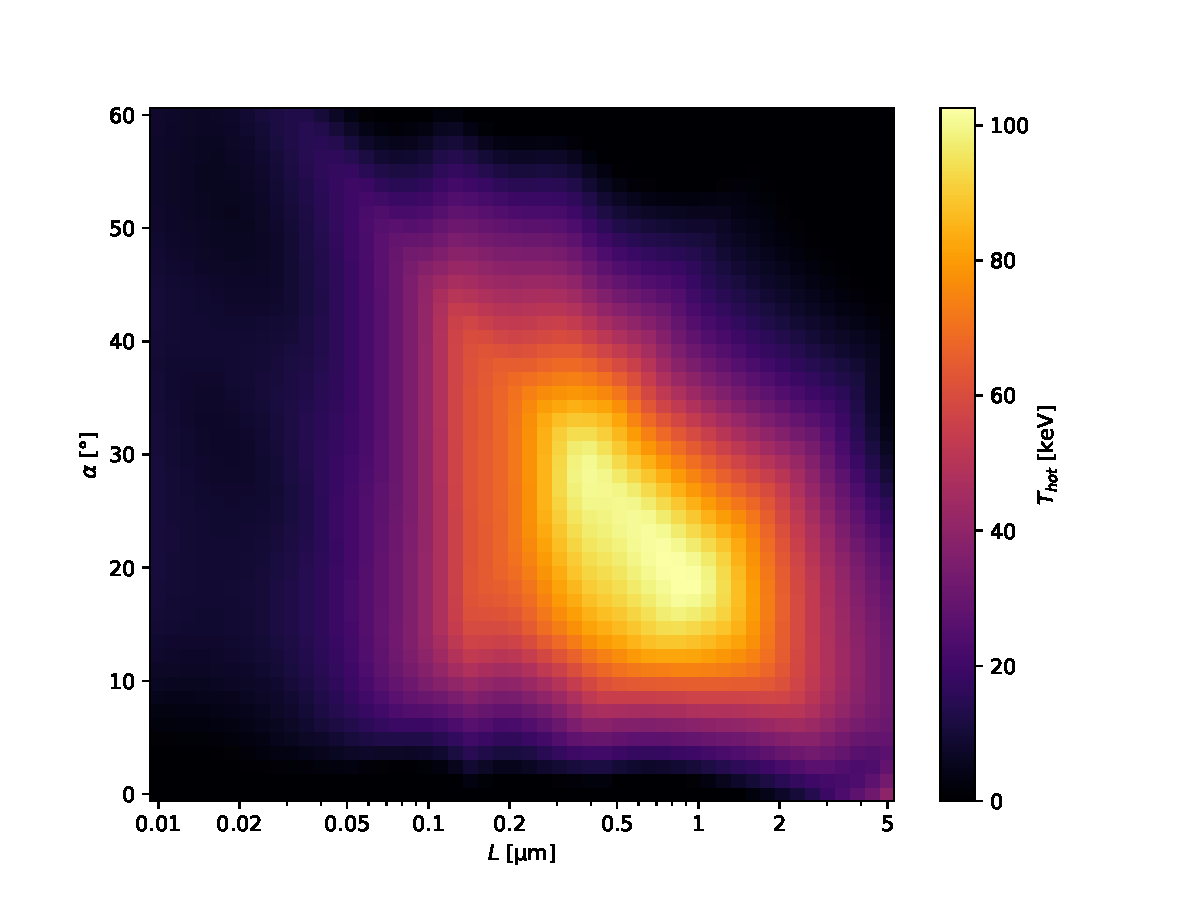
\includegraphics[width=\textwidth]{figures/nn17_pred}
		\caption{Predictions of NN model for $I = 1 \times 10^{17} \, \mathrm{W.cm}^{-2}$.}
		\label{fig:nn-pred-a}
	\end{subfigure}
	\hfill
	\begin{subfigure}{0.49\textwidth}
		\centering
		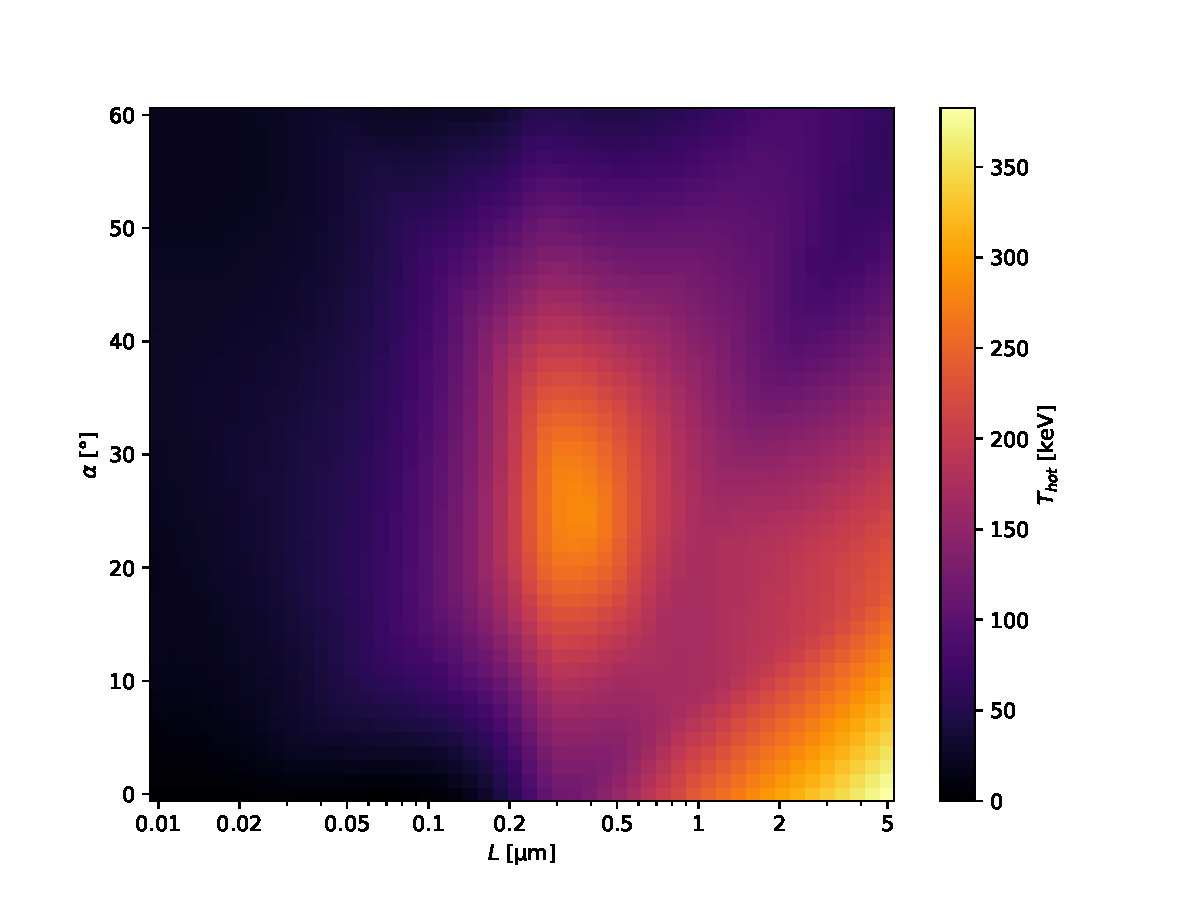
\includegraphics[width=\textwidth]{figures/nn18_pred}
		\caption{Predictions of NN model for $I = 1 \times 10^{18} \, \mathrm{W.cm}^{-2}$.}
		\label{fig:nn-pred-b}
	\end{subfigure}
	\begin{subfigure}{0.59\textwidth}
		\centering
		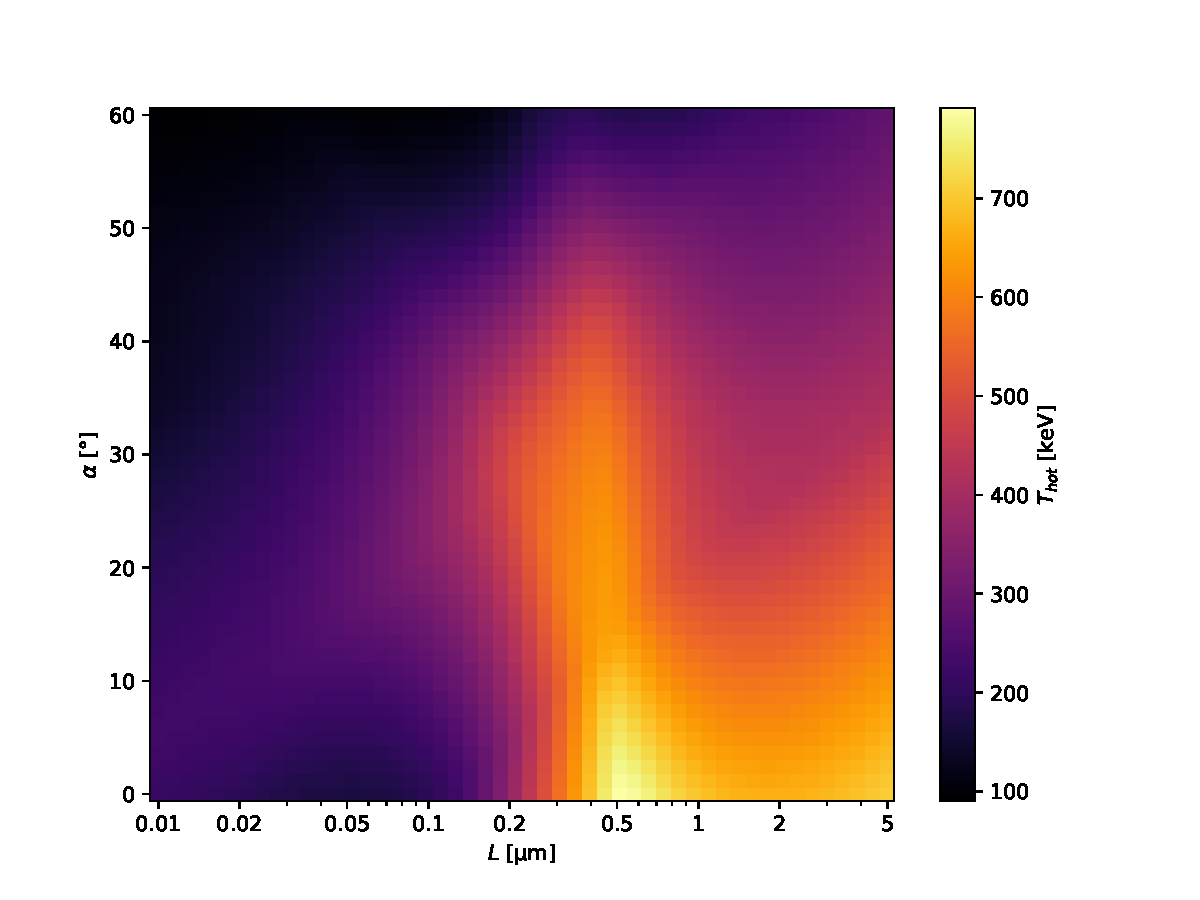
\includegraphics[width=\textwidth]{figures/nn19_pred}
		\caption{Predictions of NN model for $I = 1 \times 10^{19} \, \mathrm{W.cm}^{-2}$.}
		\label{fig:nn-pred-c}
	\end{subfigure}
	\caption{Predictions of NN model.}
	\label{fig:nn-pred}
\end{figure}

With the NN model, achieving smoothness is quite challenging because the fitting process does not explicitly account for the relationship between two data points. Regularization techniques such as weight decay and dropout do provide some improvement, though likely not as much as desired. The presence of sharp lines or ridges in the graphs indicates that the model does not generalize the relationships well enough. While further regularization could potentially increase smoothness, the results seen in the prediction graphs are probably expected given the small size of the dataset.

Despite these issues, the maxima appear to be in the correct parameter regions, and the maximum hot electron temperature is reasonably consistent with the values present in the dataset. However, it is important to note that the neural network can produce negative predictions, which do not have any physical interpretation. To address this, we decided to convert all negative predictions to zero.

Generally, it is possible to claim that the over-parametrized model can be smoothened to acceptable condition. However, it is still not completely clear, whether this architecture can capture the true physical relationship or not. The ridges, which are visible for predictions with $I = 10^{11} \, \mathrm{W.cm}^{-2}$ suggest either that we need more data, or that the total number of neurons is a little low.


\subsection*{Gaussian process regression model}
\begin{figure}[ht]
	\centering
	\begin{subfigure}{0.49\textwidth}
		\centering
		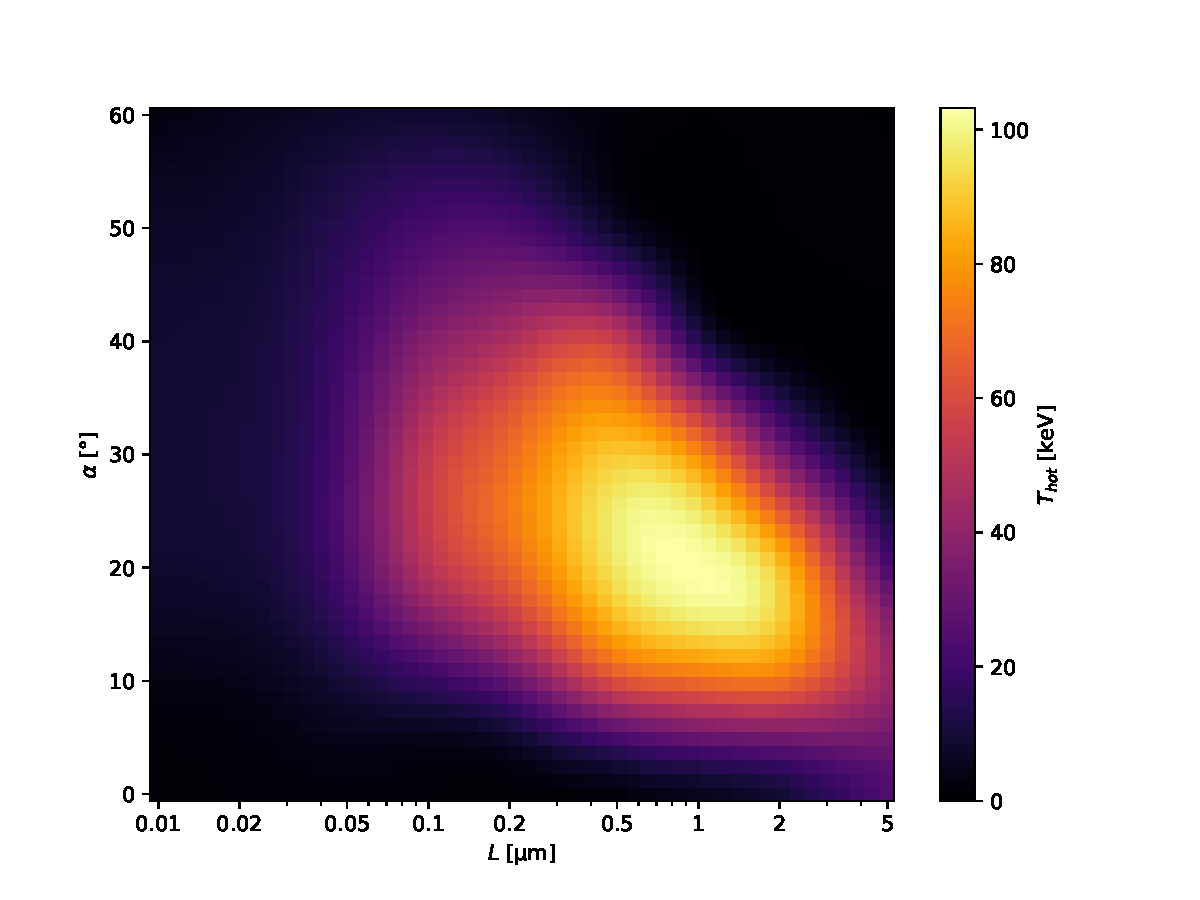
\includegraphics[width=\textwidth]{figures/gp17_pred}
		\caption{Predictions of GP model for $I = 1 \times 10^{17} \, \mathrm{W.cm}^{-2}$.}
		\label{fig:gp-pred-a}
	\end{subfigure}
	\hfill
	\begin{subfigure}{0.49\textwidth}
		\centering
		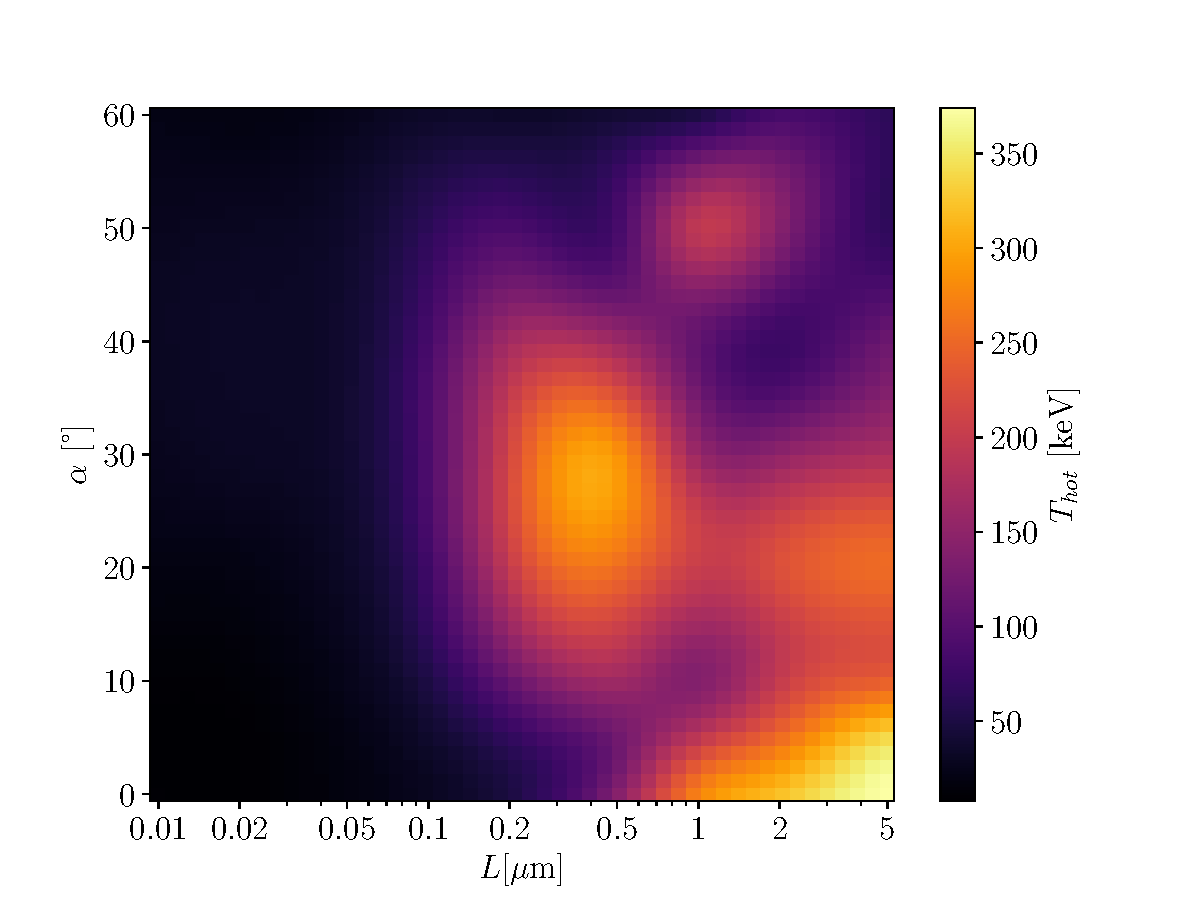
\includegraphics[width=\textwidth]{figures/gp18_pred}
		\caption{Predictions of GP model for $I = 1 \times 10^{18} \, \mathrm{W.cm}^{-2}$.}
		\label{fig:gp-pred-b}
	\end{subfigure}
	\begin{subfigure}{0.49\textwidth}
		\centering
		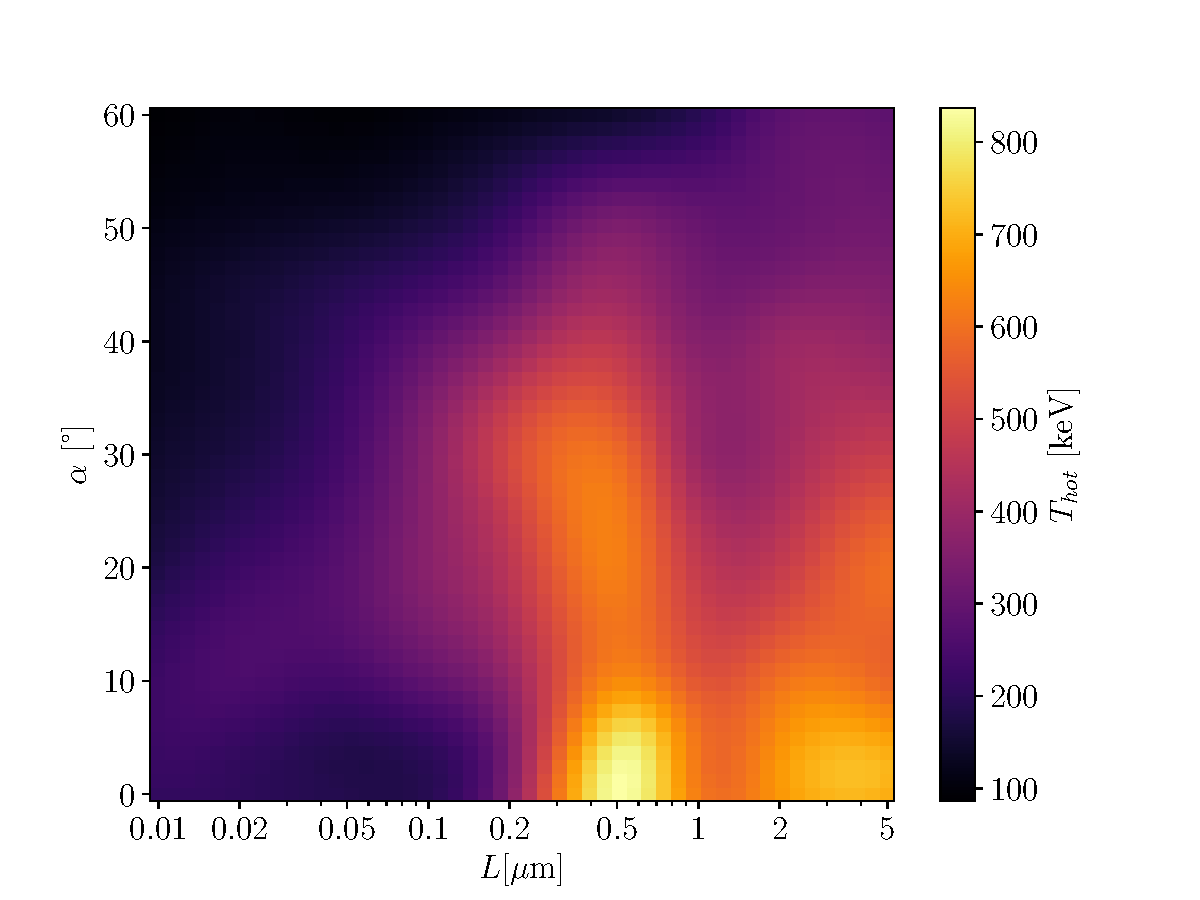
\includegraphics[width=\textwidth]{figures/gp19_pred}
		\caption{Predictions of GP model for $I = 1 \times 10^{19} \, \mathrm{W.cm}^{-2}$.}
		\label{fig:gp-pred-c}
	\end{subfigure}
	\caption{Predictions of the GP model.}
	\label{fig:gp-pred}
\end{figure}

The GP regression model has shown the best performance on the cross-validation test. Let us remind, that once the optimal parameters of the kernel are found, the predictions are calculated from the posterior distribution as it was presented in section \ref{sec:gp-theory}. The kernel parameters optimized on the whole dataset are $\sigma_k^2 =29179.49$, $l = 0.36$ and $\sigma^2 = 665.06$. The predictions shown in similar way as for NN model can be seen in figure \ref{fig:gp-pred}.

Immediately one can see, that these predictions are much smoother than those of NN model although in general, they are very similar. Probably the biggest qualitative difference can be found in the predictions for $I = 1 \times 10^{19} \, \mathrm{W.cm}^{-2}$, where the maximum temperature is lower for NN, whereas in GP the peak has almost exactly the same value as the dataset. Also, in graph for $I = 1 \times 10^{18} \, \mathrm{W.cm}^{-2}$, there is a local maximum for $\alpha = 50\degree$ and $L \approx 1 \, \mu\mathrm{m}$, which cannot be observed in the predictions of NN model.

\begin{figure}[ht]
	\centering
	\begin{subfigure}{0.49\textwidth}
		\centering
		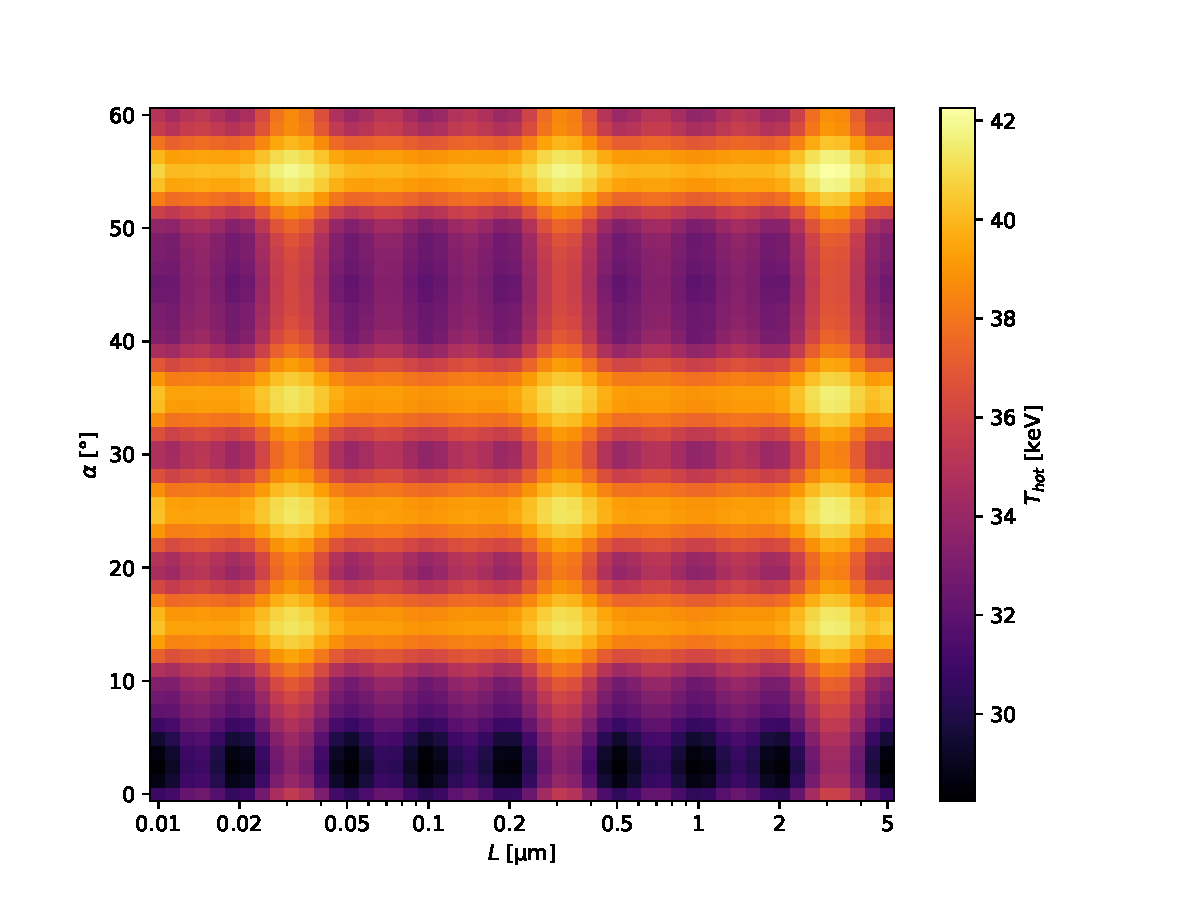
\includegraphics[width=\textwidth]{figures/gp17_pred_ss}
		\caption{Uncertainty of GP model for $I = 1 \times 10^{17} \, \mathrm{W.cm}^{-2}$.}
		\label{fig:gp-pred-ss-a}
	\end{subfigure}
	\hfill
	\begin{subfigure}{0.49\textwidth}
		\centering
		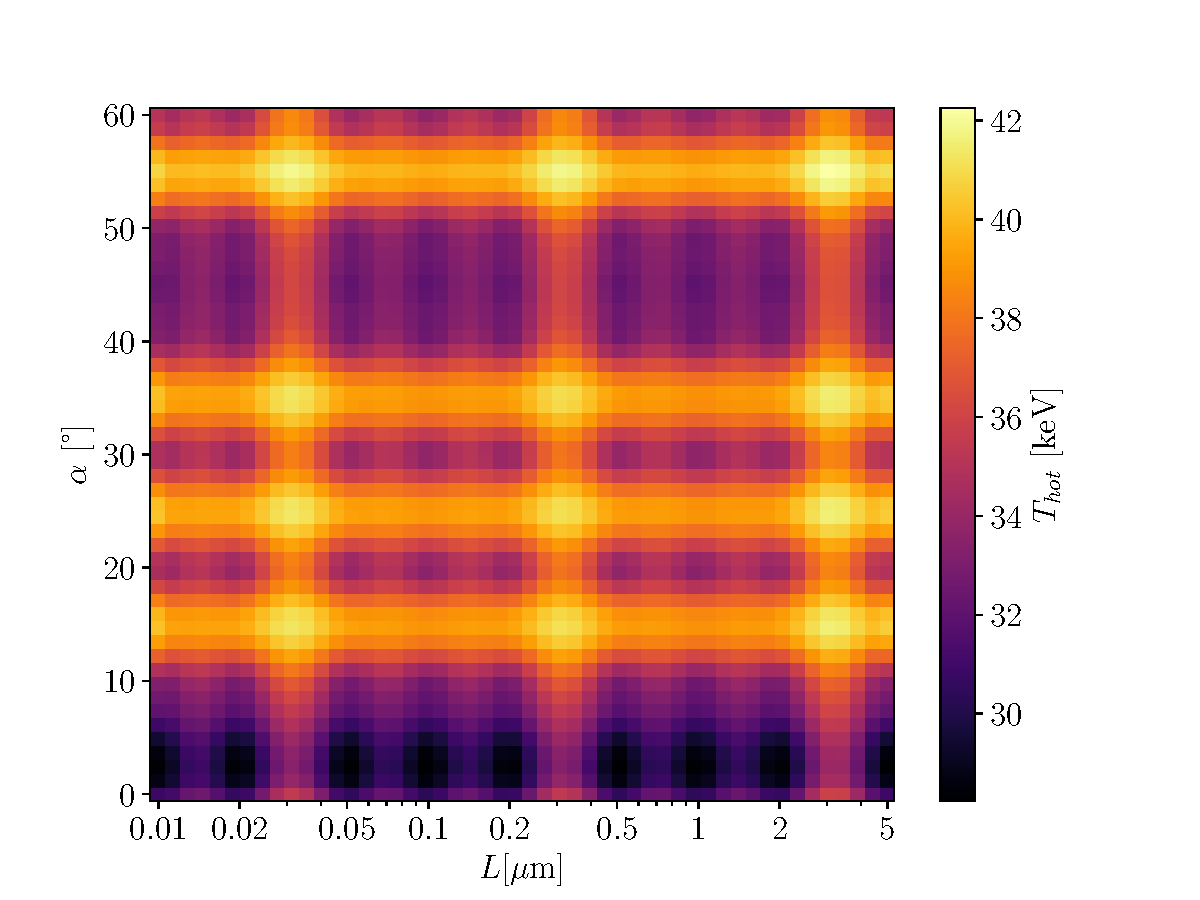
\includegraphics[width=\textwidth]{figures/gp18_pred_ss}
		\caption{Uncertainty of GP model for $I = 1 \times 10^{18} \, \mathrm{W.cm}^{-2}$.}
		\label{fig:gp-pred-ss-b}
	\end{subfigure}
	\begin{subfigure}{0.49\textwidth}
		\centering
		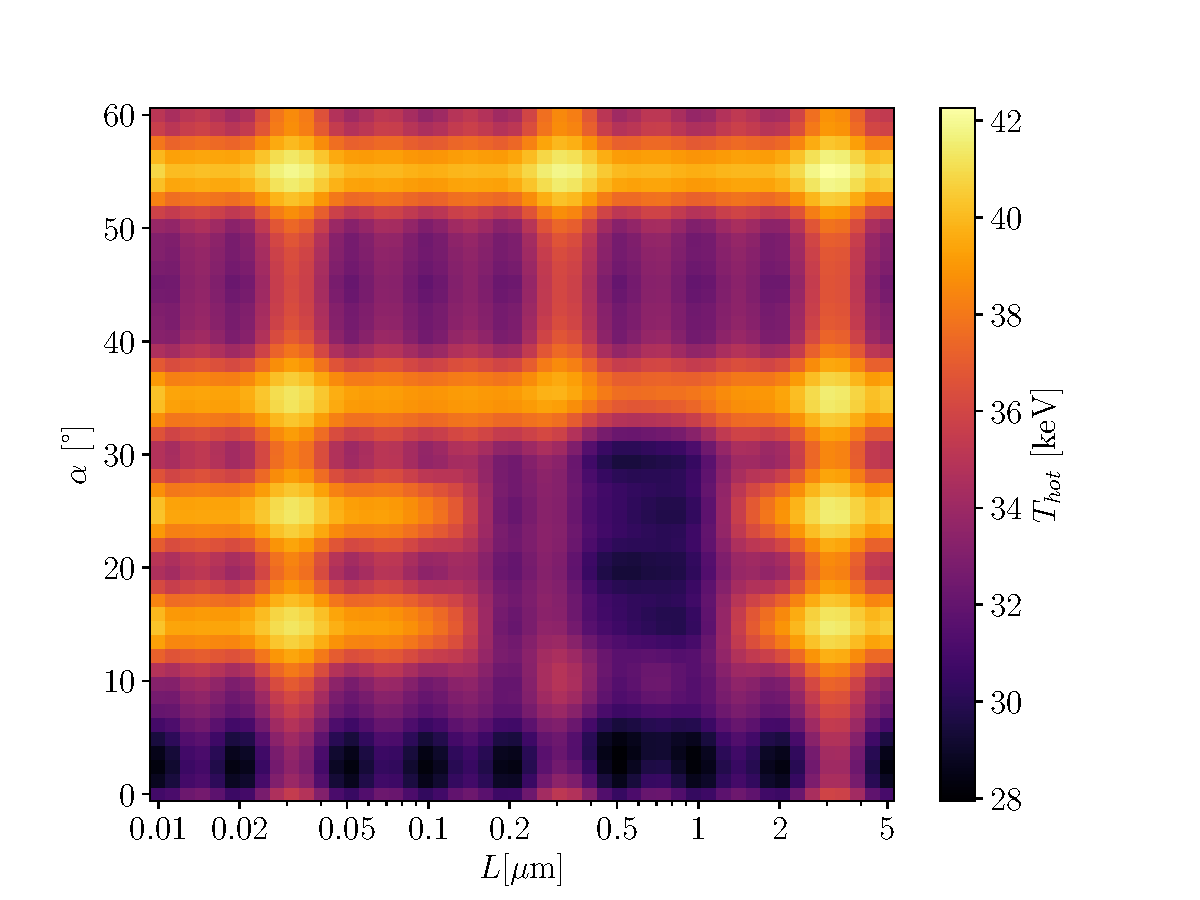
\includegraphics[width=\textwidth]{figures/gp19_pred_ss}
		\caption{Uncertainty of GP model for $I = 1 \times 10^{19} \, \mathrm{W.cm}^{-2}$.}
		\label{fig:gp-pred-ss-c}
	\end{subfigure}
	\caption{Uncertainty of the GP model.}
	\label{fig:gp-pred-ss}
\end{figure}

Now let us come back to one of the biggest strengths of the GP model. As it was stated in the section \ref{sec:gp-theory}, the GP model consists of mean function and covariance function. The predictions in \ref{fig:gp-pred} are the mean evaluated in given points. The variance of these points is calculated as diagonal elements of a matrix corresponding to the covariance function in the testing points. These values are scaled with optimized parameter of GP - noise variance $\sigma^2$. The interpretation of this parameter is therefore straightforward.

It is possible to create same plots but for the standard error $\sigma$. Such plots are shown in the figure \ref{fig:gp-pred-ss}. Naturally, the uncertainty is smaller where the training data is denser and larger in areas with sparse data. The denser the dataset, the smaller the error. The dataset was primarily created using a grid distribution of the simulation parameters. The plots hint that the dataset is denser for small angles (up to 10°), which is true. Additionally, there is a higher density of data for the intensity $I = 10^{17} \, \mathrm{W.cm}^{-2}$ around $L = 0.5\mu \mathrm{m}$ and for $\alpha$ in range of $15\degree$ to $ 30\degree$, as confirmed by the graphs.

\section{Prediction UI tool}
For the purpose of visual comparison of the models, another tool was developed. The main goal is to allow user to be able to look at the predictions of different models in different axes than those which we used until now. Plotting of custom looks can be tedious if one is writing each time a new script. Also, working with 4 dimensional data is unpleasant, because it is not possible to draw everything in one graph without sacrificing readability.

The tool provides an user interface for several basic options that are relevant for this analysis and a graph of the predictions based on the configuration. A screenshot from this application is shown in the figure \ref{fig:graph-tool}.

\begin{figure}[h]
	\centering
	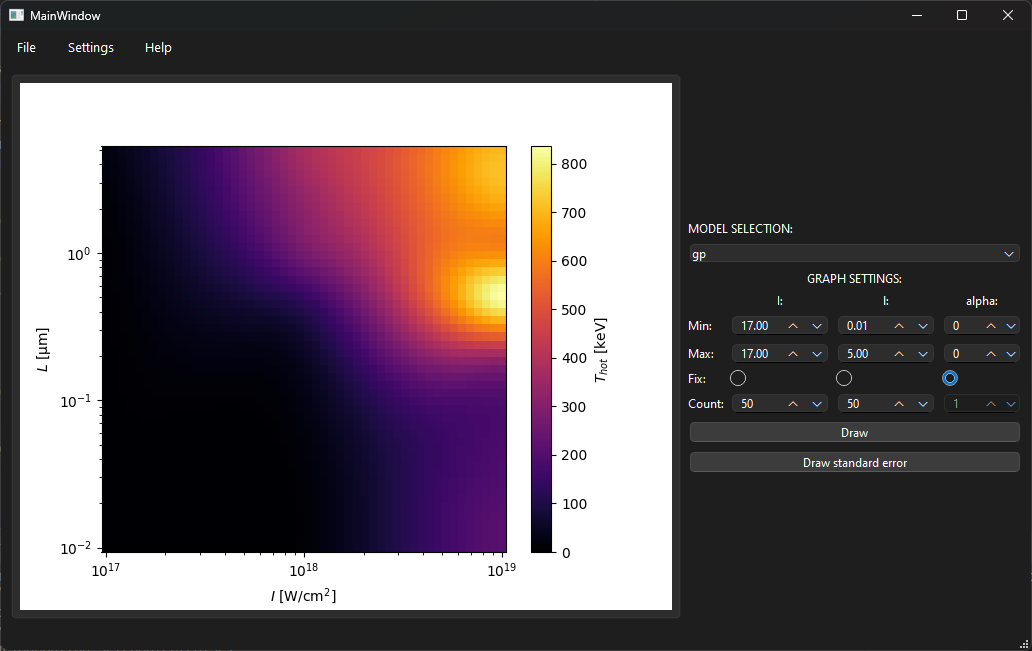
\includegraphics[width=0.85 \textwidth]{figures/graph_tool}
	\caption{A screenshot from the graphing tool with graph of GP model for $\alpha = 0\degree$.}
	\label{fig:graph-tool}
\end{figure}

The tool is quite simple, but it is tailored for this application, so it almost exhaustingly fulfils the need for special tool. It might be useful even beyond the scope of this thesis for example if someone decides to improve the models we presented or if he just wants to inspect them more closely. 

The application is implemented in Python in \textit{PyQt6} framework with the additional use of class \textit{FigureCanvasQTAgg} from \textit{matplotlib} library. The core of the functionality is relying on an abstraction, where the models are represented as a class with particular members - functions \textit{load} and \textit{predict} and already mentioned member variable of custom type \textit{Transformer}. There are also few more classes which make it easier to work with the prediction grid and the graphing canvas. Adding a support for more, completely different models is only a matter few lines of code as long s the abstraction is followed. Currently only NN, SVR and GP are supported.

\begin{figure}[h]
	\centering
	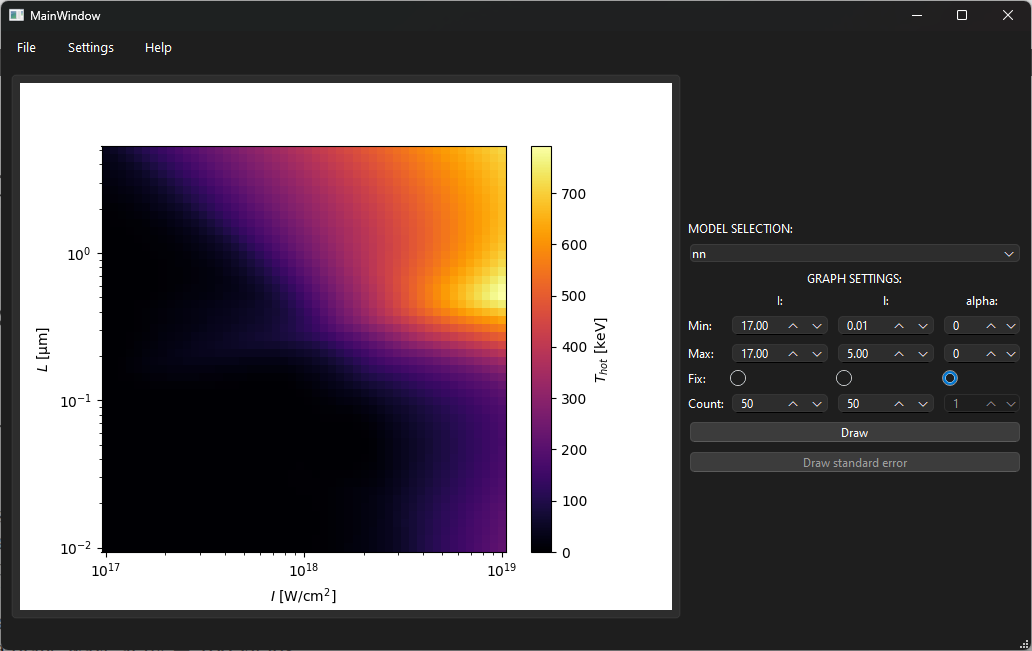
\includegraphics[width=0.85 \textwidth]{figures/graph_tool2}
	\caption{A screenshot from the graphing tool with graph of NN model for $\alpha = 0\degree$.}
	\label{fig:graph-tool2}
\end{figure}


After choosing a model, the user can choose, which axis he wants to \textit{fix} and at which value. Before, we were always fixing the intensity to three values and sampled $L$ and $\alpha$. Then, the user chooses the ranges (\textit{min}, \textit{max}) of the remaining two axes alongside with the density of the sample (\textit{count}). Prediction of the same configuration as before but for NN model is shown in the figure \ref{fig:graph-tool2}. In both examples, notice the smooth transition between the intensities. Remember that there are almost no training point off the three intensities, so the predicted temperatures could not be very accurate.

Drawing of the error is currently supported only for the GP model. By clicking the \textit{Draw standard error} button the prediction standard error is drawn. The screenshot with standard error can be seen in figure \ref{fig:graph-tool3}.
\begin{figure}[h]
	\centering
	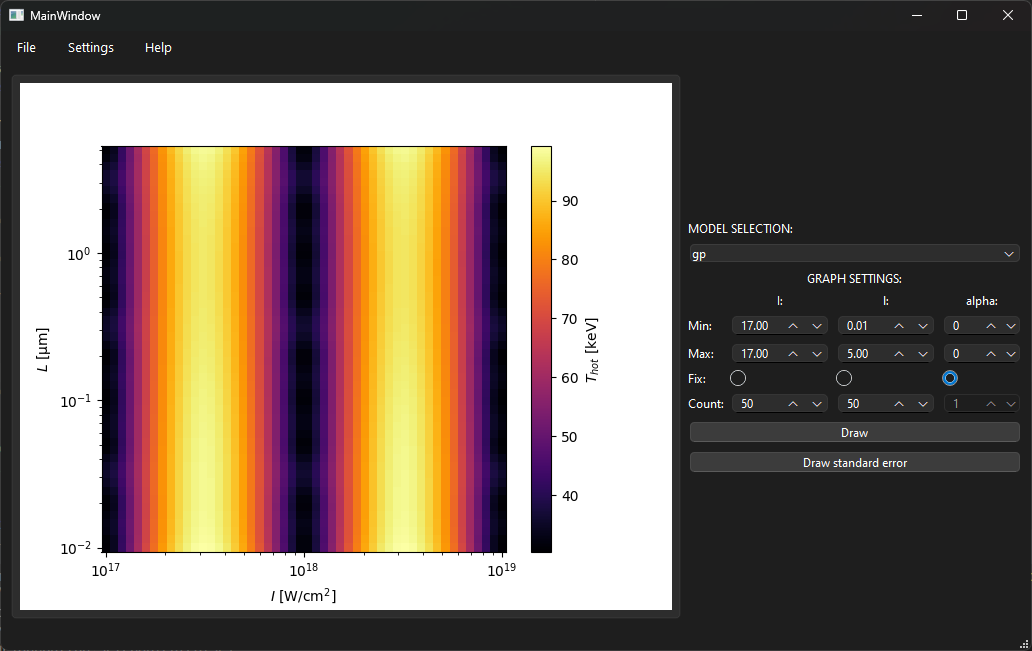
\includegraphics[width=0.85 \textwidth]{figures/graph_tool3}
	\caption{A screenshot from the graphing tool with graph of standard error of GP model for $\alpha = 0\degree$.}
	\label{fig:graph-tool3}
\end{figure}

After previous discussion, it shouldn't surprise us that the uncertainty is larger for intensities that are not a power of 10. Similar error pattern is visible when $L$ is the fixed axis, instead of $\alpha$.

\section{Strategy for choosing the next simulations}


\section{Comparison to contemporary data}
\label{ch:comparison}
In this last section, the models are compared to a few of the previous works which studied the scaling of hot electron temperature.

First, the comparison will be done with respect to work of Cui et al. \cite{cui2013}, where they model scaling of hot electron temperature with intensity using:
\begin{equation}
	content...
\end{equation}



\chapter{Comparison to contemporary data}
\chapter*{Conclusion}
\addcontentsline{toc}{chapter}{Conclusion}
%
%\input{vnitrek_zaver.tex}


%%%%%%%%%%%% SEZNAM POUŽITÝCH ZDROJŮ (LITERATURA) %%%%%%%%%%%%
\clearpage
\addcontentsline{toc}{chapter}{Seznam použitých zdrojů} % SEM NESAHEJTE!
\begin{thebibliography}{99}   
% následující text (2 řádky) zaměňte citacemi svých zdrojů
	\bibitem{odkaz} Author. \ti{Book name}. City. Publisher. Year. 
\end{thebibliography}
% formát: ČSN ISO 690. Můžete si to vygenerovat na http://www.citacepro.com (přihlaste se přes odkaz "ČVUT"), umí to vygenerovat TeX
% řazení: abecedně podle autora (resp. provního slova, není-li znám autor)


%%%%%%%%%%%% PŘÍLOHY PRÁCE %%%%%%%%%%%%
\newpage % SEM NESAHEJTE!
\addcontentsline{toc}{chapter}{Attachments} % SEM NESAHEJTE!
\appendix % SEM NESAHEJTE!


%%%%%%%%%%%% Příloha A (tj. 1. kapitola v rámci příloh) %%%%%%%%%%%%
\chapter{Attachment} % zde změňte název přílohy, příp. zakomentujte a vložte soubor, kde je název přílohy + její text (odmažte/zakomentujte text níže + odkomentujte \input{}):
Attachment
%
%\input{priloha_A.tex} % text vkládán ze souboru, kde je i příkaz \chapter{...}


\end{document} % SEM NESAHEJTE! Konec.
